\documentclass[11pt, letterpaper]{article}

% Fonts and Encoding
\usepackage[utf8]{inputenc}
\usepackage[T1]{fontenc}
\usepackage{lmodern} % High-quality Latin Modern vector font

% Math and Symbols
\usepackage{amsmath, amssymb, amsthm, amsfonts, mathrsfs, mathtools}

% Layout and Geometry
\usepackage{geometry}
\geometry{letterpaper, margin=1in}
\setlength{\parindent}{0pt}
\setlength{\parskip}{0.6em}

% Formatting and Graphics
\usepackage{graphicx, xcolor, enumitem, booktabs, array, tabularx}

% TikZ for Illustrations
\usepackage{tikz}
\usetikzlibrary{arrows.meta, positioning, shapes.geometric, calc, backgrounds, matrix}

% Clickable Links and TOC
\usepackage{hyperref}
\hypersetup{
    colorlinks=true,
    linkcolor=blue,
    filecolor=magenta,      
    urlcolor=cyan,
    pdftitle={Advanced Mathematics Topic},
}

% Theorem Environments
\newtheorem{theorem}{Theorem}[section]
\newtheorem{lemma}[theorem]{Lemma}
\newtheorem{proposition}[theorem]{Proposition}
\newtheorem{corollary}[theorem]{Corollary}
\theoremstyle{definition}
\newtheorem{definition}{Definition}[section]
\newtheorem{axiom}{Axiom}[section]
\newtheorem{example}{Example}[section]
\theoremstyle{remark}
\newtheorem{remark}{Remark}[section]

% Custom Commands (Enforced standard notation)
\newcommand{\R}{\mathbb{R}}
\newcommand{\N}{\mathbb{N}}
\newcommand{\Z}{\mathbb{Z}}
\newcommand{\Q}{\mathbb{Q}}
\newcommand{\E}{\mathbb{E}}
\newcommand{\Prob}{\mathbb{P}}
\newcommand{\F}{\mathcal{F}}

\title{\textbf{Mastery Study Guide: Section 7.2 Quadratic Forms}}
\author{Tashfeen Omran}
\date{\today}

\begin{document}

\maketitle
\tableofcontents
\newpage

% =========================================================================
% PART 1: COMPREHENSIVE INTRODUCTION, CONTEXT, AND PREREQUISITES
% =========================================================================
\section{Comprehensive Introduction, Context, and Prerequisites}

\subsection{Core Concepts and Fundamental Definitions}
Up to this point in linear algebra, the primary focus has been on linear mappings of the form $\mathbf{x} \mapsto A\mathbf{x}$ and systems of linear equations $A\mathbf{x} = \mathbf{b}$. However, across mathematics, physics, statistics, and optimization, one frequently encounters homogeneous polynomials of degree two in $n$ variables. Such expressions generalize the familiar single-variable parabola $q(x) = ax^2$ and the inner product norm squared $\|\mathbf{x}\|^2 = \mathbf{x}^T\mathbf{x} = x_1^2 + x_2^2 + \dots + x_n^2$.

\begin{definition}[Quadratic Form on $\mathbb{R}^n$]
A \textbf{quadratic form} on $\mathbb{R}^n$ is a real-valued function $Q : \mathbb{R}^n \to \mathbb{R}$ whose value at a vector $\mathbf{x} = (x_1, x_2, \dots, x_n)^T \in \mathbb{R}^n$ can be computed by an expression of the form
\[
Q(\mathbf{x}) = \mathbf{x}^T A \mathbf{x}
\]
where $A$ is an $n \times n$ \textbf{symmetric matrix} ($A^T = A$). The symmetric matrix $A$ is uniquely determined by $Q$ and is called the \textbf{matrix of the quadratic form}.
\end{definition}

When expanded in terms of coordinates $x_1, x_2, \dots, x_n$, the quadratic form $Q(\mathbf{x}) = \mathbf{x}^T A \mathbf{x}$ takes the explicit polynomial representation:
\[
Q(\mathbf{x}) = \sum_{i=1}^n \sum_{j=1}^n a_{ij} x_i x_j = \sum_{i=1}^n a_{ii} x_i^2 + 2 \sum_{1 \le i < j \le n} a_{ij} x_i x_j
\]
There are two distinct classes of terms in this polynomial:
\begin{itemize}
    \item \textbf{Square Terms ($a_{ii}x_i^2$):} The coefficient of $x_i^2$ resides directly on the $(i, i)$-diagonal entry of $A$.
    \item \textbf{Cross-Product Terms ($2a_{ij}x_ix_j$ for $i < j$):} Because $x_i x_j = x_j x_i$ for real numbers and $A$ is required to be symmetric ($a_{ij} = a_{ji}$), the coefficient $c_{ij}$ of the cross-product term $x_i x_j$ in $Q(\mathbf{x})$ is split evenly between the $(i, j)$-entry and the $(j, i)$-entry of $A$:
    \[
    a_{ij} = a_{ji} = \frac{1}{2} c_{ij}
    \]
\end{itemize}

\subsection{Intuition and Derivation of the Principal Axes Theorem}
A quadratic form without cross-product terms, such as $Q(\mathbf{y}) = \lambda_1 y_1^2 + \lambda_2 y_2^2 + \dots + \lambda_n y_n^2$, is remarkably easy to analyze: its level sets are aligned with the coordinate axes, and the range of values $Q(\mathbf{y})$ can take is immediately visible from the signs of the coefficients $\lambda_1, \dots, \lambda_n$. In contrast, when cross-product terms $x_i x_j$ ($i \neq j$) are present, the geometric level sets $\mathbf{x}^T A \mathbf{x} = c$ are rotated out of standard position, and the sign behavior of $Q(\mathbf{x})$ is obscured. For instance, in Example 6 of the text, the form
\[
Q(\mathbf{x}) = 3x_1^2 + 2x_2^2 + x_3^2 + 4x_1x_2 + 4x_2x_3
\]
has exclusively positive coefficients, yet it takes negative values (e.g., at $\mathbf{x} = (1, -2, 2)^T$, $Q(\mathbf{x}) = 3(1) + 2(4) + 1(4) + 4(-2) + 4(-4) = 15 - 24 = -9$).

To eliminate cross-product terms, we introduce a linear \textbf{change of variable}:
\[
\mathbf{x} = P\mathbf{y} \quad \Longleftrightarrow \quad \mathbf{y} = P^{-1}\mathbf{x}
\]
where $P$ is an invertible $n \times n$ matrix and $\mathbf{y} \in \mathbb{R}^n$ represents the coordinate vector of $\mathbf{x}$ relative to the basis formed by the columns of $P$. Substituting $\mathbf{x} = P\mathbf{y}$ into $Q(\mathbf{x})$ and applying the transpose rule $(P\mathbf{y})^T = \mathbf{y}^T P^T$, we derive:
\[
Q(\mathbf{x}) = \mathbf{x}^T A \mathbf{x} = (P\mathbf{y})^T A (P\mathbf{y}) = \mathbf{y}^T P^T A P \mathbf{y} = \mathbf{y}^T (P^T A P) \mathbf{y}
\]
Thus, in terms of the new variable $\mathbf{y}$, the matrix of the quadratic form is $P^T A P$. Because $A$ is symmetric, the Spectral Theorem (Section 7.1, Theorem 2) guarantees that $A$ is orthogonally diagonalizable: there exists an orthogonal matrix $P$ (meaning $P^T = P^{-1}$) whose columns $\mathbf{u}_1, \dots, \mathbf{u}_n$ form an orthonormal basis of eigenvectors of $A$, such that
\[
P^T A P = P^{-1} A P = D = \operatorname{diag}(\lambda_1, \lambda_2, \dots, \lambda_n)
\]
Under this orthogonal change of variable $\mathbf{x} = P\mathbf{y}$, the quadratic form simplifies completely into a pure sum of squares weighted by the eigenvalues of $A$:
\[
\mathbf{x}^T A \mathbf{x} = \mathbf{y}^T D \mathbf{y} = \lambda_1 y_1^2 + \lambda_2 y_2^2 + \dots + \lambda_n y_n^2
\]

\begin{theorem}[Theorem 4: The Principal Axes Theorem]
Let $A$ be an $n \times n$ symmetric matrix. Then there is an orthogonal change of variable, $\mathbf{x} = P\mathbf{y}$, that transforms the quadratic form $\mathbf{x}^T A \mathbf{x}$ into a quadratic form $\mathbf{y}^T D \mathbf{y}$ with no cross-product term. The columns of $P$ are called the \textbf{principal axes} of the quadratic form $\mathbf{x}^T A \mathbf{x}$.
\end{theorem}

\begin{center}
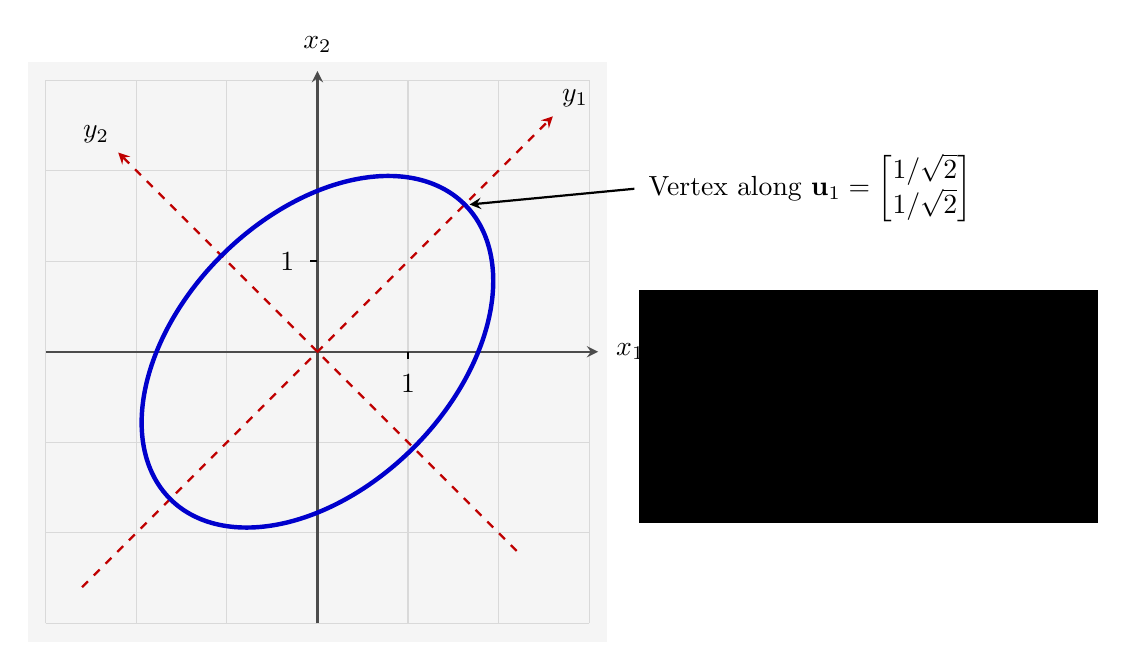
\begin{tikzpicture}[scale=1.15]
    % 1. Background fills
    \fill[gray!8] (-3.2,-3.2) rectangle (3.2,3.2);
    
    % 2. Grid lines and Original Axes
    \draw[step=1.0, gray!30, thin] (-3,-3) grid (3,3);
    \draw[->, >=stealth, thick, black!70] (-3,0) -- (3.1,0);
    \draw[->, >=stealth, thick, black!70] (0,-3) -- (0,3.1);
    
    % Rotated Principal Axes (y1, y2 at 45 degrees for 5x1^2 - 4x1x2 + 5x2^2 = 48, scaled)
    \draw[->, >=stealth, thick, red!75!black, dashed] (-2.6,-2.6) -- (2.6,2.6);
    \draw[->, >=stealth, thick, red!75!black, dashed] (2.2,-2.2) -- (-2.2,2.2);
    
    % 3. Primary Plot: Rotated Ellipse
    % Using parametric form in principal axes: y1 = a cos(t), y2 = b sin(t) rotated by 45 deg
    \draw[ultra thick, blue!80!black, samples=120, domain=0:360, smooth, variable=\t] 
        plot ({2.3*cos(\t)*0.7071 - 1.5*sin(\t)*0.7071}, {2.3*cos(\t)*0.7071 + 1.5*sin(\t)*0.7071});
        
    % Callout arrows
    \draw[->, >=stealth, shorten >=2pt, thick, black] (3.5, 1.8) -- (1.62, 1.62);
    
    % 4. Node Labels and Single-Node Legend
    \node[right=3pt, black] at (3.1,0) {$x_1$};
    \node[above=3pt, black] at (0,3.1) {$x_2$};
    \node[above right=2pt, black] at (2.55,2.55) {$y_1$};
    \node[above left=2pt, black] at (-2.15,2.15) {$y_2$};
    
    \draw[thick, black] (1,0) -- (1,-0.08) node[below=2pt, black] {$1$};
    \draw[thick, black] (0,1) -- (-0.08,1) node[left=2pt, black] {$1$};
    
    \node[align=left, anchor=west, black] at (3.55, 1.8) {$\displaystyle \text{Vertex along } \mathbf{u}_1 = \begin{bmatrix} 1/\sqrt{2} \\ 1/\sqrt{2} \end{bmatrix}$};
    
    \node[draw=black!60, fill=white, inner sep=8pt, align=left, anchor=west, black] at (3.55, -0.6) {
        \textbf{Geometric Principal Axes}\\[4pt]
        $\displaystyle \text{Original: } 5x_1^2 - 4x_1x_2 + 5x_2^2 = 48$\\[2pt]
        $\displaystyle \text{Principal Axes: } 3y_1^2 + 7y_2^2 = 48$\\[2pt]
        $\displaystyle P = \begin{bmatrix} \mathbf{u}_1 & \mathbf{u}_2 \end{bmatrix} = \begin{bmatrix} 1/\sqrt{2} & -1/\sqrt{2} \\ 1/\sqrt{2} & 1/\sqrt{2} \end{bmatrix}$
    };
\end{tikzpicture}
\end{center}

\subsection{Historical Context and Motivation}
The systematic theory of quadratic forms originated in the 18th and 19th centuries through two converging streams of inquiry: celestial mechanics and number theory. In analytical mechanics and geometry, Leonhard Euler (1748) and Joseph-Louis Lagrange (1759) investigated the classification of quadric surfaces in three-dimensional space (such as ellipsoids and hyperboloids) and the moment of inertia tensor of rigid bodies, discovering that any quadric surface can be rotated onto three mutually perpendicular principal axes. In the 1820s, Augustin-Louis Cauchy formalized this rotation algebraically by proving that the characteristic roots (eigenvalues) of a real symmetric matrix are always real and that its eigenvectors determine orthogonal principal axes.

Simultaneously, Carl Friedrich Gauss (in \textit{Disquisitiones Arithmeticae}, 1801), Carl Gustav Jacob Jacobi, and James Joseph Sylvester developed the algebraic invariants of quadratic forms, introducing the concepts of definiteness and Sylvester's Law of Inertia. This framework became the mathematical bedrock for Riemannian geometry (where the metric tensor $ds^2 = \sum g_{ij} dx_i dx_j$ is a positive definite quadratic form at each point), multivariable calculus (where the second-derivative Hessian test relies entirely on the definiteness of the Hessian quadratic form), and modern multivariate statistics (where the Mahalanobis distance and Gaussian probability density contours are governed by the inverse covariance quadratic form).

\subsection{Classification of Quadratic Forms and Key Formulas}
\begin{definition}[Definiteness of Quadratic Forms]
Let $Q : \mathbb{R}^n \to \mathbb{R}$ be a quadratic form given by $Q(\mathbf{x}) = \mathbf{x}^T A \mathbf{x}$ with $A^T = A$. Then $Q$ (and by extension the symmetric matrix $A$) is classified as:
\begin{enumerate}[label=\alph*.]
    \item \textbf{Positive definite} if $Q(\mathbf{x}) > 0$ for all $\mathbf{x} \neq \mathbf{0}$.
    \item \textbf{Negative definite} if $Q(\mathbf{x}) < 0$ for all $\mathbf{x} \neq \mathbf{0}$.
    \item \textbf{Indefinite} if $Q(\mathbf{x})$ assumes both strictly positive and strictly negative values.
    \item \textbf{Positive semidefinite} if $Q(\mathbf{x}) \ge 0$ for all $\mathbf{x} \in \mathbb{R}^n$.
    \item \textbf{Negative semidefinite} if $Q(\mathbf{x}) \le 0$ for all $\mathbf{x} \in \mathbb{R}^n$.
\end{enumerate}
\end{definition}

\begin{theorem}[Theorem 5: Quadratic Forms and Eigenvalues]
Let $A$ be an $n \times n$ symmetric matrix. Then a quadratic form $\mathbf{x}^T A \mathbf{x}$ is:
\begin{enumerate}[label=\alph*.]
    \item \textbf{positive definite} if and only if the eigenvalues of $A$ are all strictly positive ($\lambda_i > 0$ for all $i$),
    \item \textbf{negative definite} if and only if the eigenvalues of $A$ are all strictly negative ($\lambda_i < 0$ for all $i$), or
    \item \textbf{indefinite} if and only if $A$ has both strictly positive and strictly negative eigenvalues.
\end{enumerate}
Furthermore, $\mathbf{x}^T A \mathbf{x}$ is \textbf{positive semidefinite} if and only if all eigenvalues satisfy $\lambda_i \ge 0$, and \textbf{negative semidefinite} if and only if all eigenvalues satisfy $\lambda_i \le 0$.
\end{theorem}

\renewcommand{\arraystretch}{1.5}
\begin{tabularx}{\textwidth}{>{$\displaystyle}l<{$} >{$\displaystyle}c<{$} X}
\toprule
\textbf{Concept} & \textbf{Formula / Characterization} & \textbf{Description} \\
\midrule
\text{Matrix Entry Rule} & a_{ii} = \text{coeff of } x_i^2, \quad a_{ij} = a_{ji} = \frac{1}{2}(\text{coeff of } x_ix_j) & Converts polynomial $Q(\mathbf{x})$ to symmetric $A$. \\
\text{Change of Variable} & \mathbf{x} = P\mathbf{y} \iff \mathbf{y} = P^T \mathbf{x} \quad (P \text{ orthogonal}) & Maps principal-axis coordinates $\mathbf{y}$ to $\mathbf{x}$. \\
\text{Diagonalized Form} & \mathbf{x}^T A \mathbf{x} = \mathbf{y}^T (P^T A P) \mathbf{y} = \sum_{i=1}^n \lambda_i y_i^2 & Eliminates all cross-product terms $y_i y_j$. \\
\text{Cholesky Factorization} & A = R^T R \quad (R \text{ upper triangular, } r_{ii} > 0) & Exists if and only if $A$ is positive definite. \\
2\times 2 \text{ Det/Trace Test} & \det A = \lambda_1\lambda_2, \quad \operatorname{tr}(A) = a+d = \lambda_1+\lambda_2 & Classifies $2\times 2$ forms without eigenvalues. \\
\bottomrule
\end{tabularx}

\subsection{Prerequisites}
To master Section 7.2, you must be fluent in the following foundational concepts:
\begin{enumerate}
    \item \textbf{Matrix Multiplication and Transposes (Section 2.1):} Computing row-by-matrix-by-column products $\mathbf{x}^T A \mathbf{x}$ and applying the reversal law $(AB)^T = B^T A^T$.
    \item \textbf{Characteristic Polynomials and Eigenvalues (Section 5.2):} Solving $\det(A - \lambda I) = 0$ and finding bases for eigenspaces $\operatorname{Nul}(A - \lambda I)$.
    \item \textbf{Orthogonal Sets, Orthonormal Bases, and the Gram-Schmidt Process (Sections 6.2--6.4):} Normalizing vectors $\mathbf{u} = \mathbf{v}/\|\mathbf{v}\|$ and constructing orthogonal bases for multidimensional eigenspaces when an eigenvalue has multiplicity greater than $1$.
    \item \textbf{Orthogonal Diagonalization of Symmetric Matrices (Section 7.1):} Constructing an orthogonal matrix $P = \begin{bmatrix} \mathbf{u}_1 & \dots & \mathbf{u}_n \end{bmatrix}$ such that $P^T A P = D$, using the fact that eigenvectors from distinct eigenspaces of a symmetric matrix are automatically orthogonal.
\end{enumerate}

\newpage
% =========================================================================
% PART 2: DETAILED HOMEWORK SOLUTIONS
% =========================================================================
\section{Detailed Homework Solutions}

\subsection*{Practice Problem}
\textbf{Original Problem:} Describe a positive semidefinite matrix $A$ in terms of its eigenvalues.

\textbf{Solution:}
A symmetric $n \times n$ matrix $A$ is positive semidefinite if and only if all of its eigenvalues are nonnegative ($\lambda_i \ge 0$ for all $i = 1, 2, \dots, n$).

\textit{Proof:} By the Principal Axes Theorem (Theorem 4), there exists an orthogonal change of variable $\mathbf{x} = P\mathbf{y}$ such that
\[
Q(\mathbf{x}) = \mathbf{x}^T A \mathbf{x} = \mathbf{y}^T D \mathbf{y} = \lambda_1 y_1^2 + \lambda_2 y_2^2 + \dots + \lambda_n y_n^2
\]
where $\lambda_1, \lambda_2, \dots, \lambda_n$ are the eigenvalues of $A$.
\begin{itemize}
    \item ($\Rightarrow$) Suppose $A$ is positive semidefinite, so $\mathbf{x}^T A \mathbf{x} \ge 0$ for all $\mathbf{x} \in \mathbb{R}^n$. If any eigenvalue $\lambda_i$ were strictly negative ($\lambda_i < 0$), then choosing $\mathbf{y} = \mathbf{e}_i$ (the $i$-th standard basis vector of $\mathbb{R}^n$, corresponding to $\mathbf{x} = P\mathbf{e}_i$) would yield
    \[
    \mathbf{x}^T A \mathbf{x} = \lambda_i (1)^2 = \lambda_i < 0
    \]
    which contradicts $\mathbf{x}^T A \mathbf{x} \ge 0$. Thus, every eigenvalue of $A$ must satisfy $\lambda_i \ge 0$.
    \item ($\Leftarrow$) Conversely, if $\lambda_i \ge 0$ for all $i = 1, \dots, n$, then since $y_i^2 \ge 0$ for every real number $y_i$, every term $\lambda_i y_i^2 \ge 0$. Therefore, $\mathbf{x}^T A \mathbf{x} = \sum_{i=1}^n \lambda_i y_i^2 \ge 0$ for all $\mathbf{x} \in \mathbb{R}^n$, proving that $A$ is positive semidefinite.
\end{itemize}
\textbf{Final Answer:} A symmetric matrix $A$ is positive semidefinite if and only if all of its eigenvalues are nonnegative ($\lambda_i \ge 0$).

\medskip\hrule\medskip

\subsection*{Exercise 1}
\textbf{Original Problem:} Compute the quadratic form $\mathbf{x}^T A \mathbf{x}$, when $A = \begin{bmatrix} 3 & 1/4 \\ 1/4 & 1 \end{bmatrix}$ and
\begin{enumerate}[label=\alph*.]
    \item $\mathbf{x} = \begin{bmatrix} x_1 \\ x_2 \end{bmatrix}$
    \item $\mathbf{x} = \begin{bmatrix} 8 \\ 1 \end{bmatrix}$
    \item $\mathbf{x} = \begin{bmatrix} 1 \\ 4 \end{bmatrix}$
\end{enumerate}

\textbf{Solution:}
\begin{enumerate}[label=\alph*.]
    \item For $\mathbf{x} = \begin{bmatrix} x_1 \\ x_2 \end{bmatrix}$, we first compute the matrix-vector product $A\mathbf{x}$ and then multiply on the left by $\mathbf{x}^T$:
    \begin{align*}
        \mathbf{x}^T A \mathbf{x} &= \begin{bmatrix} x_1 & x_2 \end{bmatrix} \begin{bmatrix} 3 & 1/4 \\ 1/4 & 1 \end{bmatrix} \begin{bmatrix} x_1 \\ x_2 \end{bmatrix} \\
        &= \begin{bmatrix} x_1 & x_2 \end{bmatrix} \begin{bmatrix} 3x_1 + \frac{1}{4}x_2 \\[4pt] \frac{1}{4}x_1 + x_2 \end{bmatrix} \\
        &= x_1\left(3x_1 + \frac{1}{4}x_2\right) + x_2\left(\frac{1}{4}x_1 + x_2\right) \\
        &= 3x_1^2 + \frac{1}{4}x_1x_2 + \frac{1}{4}x_2x_1 + x_2^2 \\
        &= 3x_1^2 + \frac{1}{2}x_1x_2 + x_2^2
    \end{align*}
    \textbf{Final Answer (a):} $3x_1^2 + \frac{1}{2}x_1x_2 + x_2^2$

    \item For $\mathbf{x} = \begin{bmatrix} 8 \\ 1 \end{bmatrix}$, we can either multiply the matrices directly or substitute $x_1 = 8, x_2 = 1$ into the polynomial from part (a):
    \begin{align*}
        \mathbf{x}^T A \mathbf{x} &= \begin{bmatrix} 8 & 1 \end{bmatrix} \begin{bmatrix} 3 & 1/4 \\ 1/4 & 1 \end{bmatrix} \begin{bmatrix} 8 \\ 1 \end{bmatrix} = \begin{bmatrix} 8 & 1 \end{bmatrix} \begin{bmatrix} 24 + 1/4 \\ 2 + 1 \end{bmatrix} \\
        &= 8\left(\frac{97}{4}\right) + 1(3) = 194 + 3 = 197
    \end{align*}
    Checking via part (a): $3(8)^2 + \frac{1}{2}(8)(1) + (1)^2 = 3(64) + 4 + 1 = 192 + 5 = 197$.
    
    \textbf{Final Answer (b):} $197$

    \item For $\mathbf{x} = \begin{bmatrix} 1 \\ 4 \end{bmatrix}$, we compute:
    \begin{align*}
        \mathbf{x}^T A \mathbf{x} &= \begin{bmatrix} 1 & 4 \end{bmatrix} \begin{bmatrix} 3 & 1/4 \\ 1/4 & 1 \end{bmatrix} \begin{bmatrix} 1 \\ 4 \end{bmatrix} = \begin{bmatrix} 1 & 4 \end{bmatrix} \begin{bmatrix} 3 + 1 \\ 1/4 + 4 \end{bmatrix} \\
        &= 1(4) + 4\left(\frac{17}{4}\right) = 4 + 17 = 21
    \end{align*}
    Checking via part (a): $3(1)^2 + \frac{1}{2}(1)(4) + (4)^2 = 3 + 2 + 16 = 21$.
    
    \textbf{Final Answer (c):} $21$
\end{enumerate}

\medskip\hrule\medskip

\subsection*{Exercise 2}
\textbf{Original Problem:} Compute the quadratic form $\mathbf{x}^T A \mathbf{x}$, for $A = \begin{bmatrix} 4 & 1 & 0 \\ 1 & 1 & 3 \\ 0 & 3 & 0 \end{bmatrix}$ and
\begin{enumerate}[label=\alph*.]
    \item $\mathbf{x} = \begin{bmatrix} x_1 \\ x_2 \\ x_3 \end{bmatrix}$
    \item $\mathbf{x} = \begin{bmatrix} -3 \\ -1 \\ 4 \end{bmatrix}$
    \item $\mathbf{x} = \begin{bmatrix} 1/\sqrt{5} \\ 1/\sqrt{5} \\ 1/\sqrt{5} \end{bmatrix}$
\end{enumerate}

\textbf{Solution:}
\begin{enumerate}[label=\alph*.]
    \item For $\mathbf{x} = \begin{bmatrix} x_1 \\ x_2 \\ x_3 \end{bmatrix}$, we compute:
    \begin{align*}
        \mathbf{x}^T A \mathbf{x} &= \begin{bmatrix} x_1 & x_2 & x_3 \end{bmatrix} \begin{bmatrix} 4 & 1 & 0 \\ 1 & 1 & 3 \\ 0 & 3 & 0 \end{bmatrix} \begin{bmatrix} x_1 \\ x_2 \\ x_3 \end{bmatrix} \\
        &= \begin{bmatrix} x_1 & x_2 & x_3 \end{bmatrix} \begin{bmatrix} 4x_1 + x_2 \\ x_1 + x_2 + 3x_3 \\ 3x_2 \end{bmatrix} \\
        &= x_1(4x_1 + x_2) + x_2(x_1 + x_2 + 3x_3) + x_3(3x_2) \\
        &= 4x_1^2 + x_1x_2 + x_2x_1 + x_2^2 + 3x_2x_3 + 3x_3x_2 \\
        &= 4x_1^2 + x_2^2 + 2x_1x_2 + 6x_2x_3
    \end{align*}
    \textbf{Final Answer (a):} $4x_1^2 + x_2^2 + 2x_1x_2 + 6x_2x_3$

    \item For $\mathbf{x} = \begin{bmatrix} -3 \\ -1 \\ 4 \end{bmatrix}$, substituting $x_1 = -3$, $x_2 = -1$, $x_3 = 4$ into the formula from part (a) (or multiplying directly):
    \begin{align*}
        \mathbf{x}^T A \mathbf{x} &= 4(-3)^2 + (-1)^2 + 2(-3)(-1) + 6(-1)(4) \\
        &= 4(9) + 1 + 6 - 24 = 36 + 7 - 24 = 19
    \end{align*}
    \textbf{Final Answer (b):} $19$

    \item For $\mathbf{x} = \begin{bmatrix} 1/\sqrt{5} \\ 1/\sqrt{5} \\ 1/\sqrt{5} \end{bmatrix}$, note that $x_i x_j = \left(\frac{1}{\sqrt{5}}\right)^2 = \frac{1}{5}$ for all $i, j \in \{1, 2, 3\}$. Thus:
    \begin{align*}
        \mathbf{x}^T A \mathbf{x} &= 4\left(\frac{1}{5}\right) + 1\left(\frac{1}{5}\right) + 2\left(\frac{1}{5}\right) + 6\left(\frac{1}{5}\right) \\
        &= \frac{4 + 1 + 2 + 6}{5} = \frac{13}{5}
    \end{align*}
    \textbf{Final Answer (c):} $\dfrac{13}{5}$
\end{enumerate}

\medskip\hrule\medskip

\subsection*{Exercise 3}
\textbf{Original Problem:} Find the matrix of the quadratic form. Assume $\mathbf{x}$ is in $\mathbb{R}^2$.
\begin{enumerate}[label=\alph*.]
    \item $4x_1^2 - 6x_1x_2 + 5x_2^2$
    \item $5x_1^2 + 4x_1x_2$
\end{enumerate}

\textbf{Solution:}
\begin{enumerate}[label=\alph*.]
    \item Place the coefficients of $x_1^2$ and $x_2^2$ ($4$ and $5$) on the main diagonal, and split the cross-product coefficient $-6$ evenly between $a_{12}$ and $a_{21}$ ($-6/2 = -3$):
    \[
    A = \begin{bmatrix} 4 & -3 \\ -3 & 5 \end{bmatrix}
    \]
    \textbf{Final Answer (a):} $\begin{bmatrix} 4 & -3 \\ -3 & 5 \end{bmatrix}$

    \item The coefficient of $x_1^2$ is $5$ and the coefficient of $x_2^2$ is $0$. Splitting the cross-product coefficient $4$ evenly gives $a_{12} = a_{21} = 4/2 = 2$:
    \[
    A = \begin{bmatrix} 5 & 2 \\ 2 & 0 \end{bmatrix}
    \]
    \textbf{Final Answer (b):} $\begin{bmatrix} 5 & 2 \\ 2 & 0 \end{bmatrix}$
\end{enumerate}

\medskip\hrule\medskip

\subsection*{Exercise 4}
\textbf{Original Problem:} Find the matrix of the quadratic form. Assume $\mathbf{x}$ is in $\mathbb{R}^2$.
\begin{enumerate}[label=\alph*.]
    \item $7x_1^2 + 18x_1x_2 - 7x_2^2$
    \item $8x_1x_2$
\end{enumerate}

\textbf{Solution:}
\begin{enumerate}[label=\alph*.]
    \item Place $7$ and $-7$ on the main diagonal, and split $18$ evenly between $a_{12}$ and $a_{21}$ ($18/2 = 9$):
    \[
    A = \begin{bmatrix} 7 & 9 \\ 9 & -7 \end{bmatrix}
    \]
    \textbf{Final Answer (a):} $\begin{bmatrix} 7 & 9 \\ 9 & -7 \end{bmatrix}$

    \item Both squared terms $x_1^2$ and $x_2^2$ have coefficient $0$. Splitting the cross-product coefficient $8$ evenly gives $a_{12} = a_{21} = 8/2 = 4$:
    \[
    A = \begin{bmatrix} 0 & 4 \\ 4 & 0 \end{bmatrix}
    \]
    \textbf{Final Answer (b):} $\begin{bmatrix} 0 & 4 \\ 4 & 0 \end{bmatrix}$
\end{enumerate}

\medskip\hrule\medskip

\subsection*{Exercise 5}
\textbf{Original Problem:} Find the matrix of the quadratic form. Assume $\mathbf{x}$ is in $\mathbb{R}^3$.
\begin{enumerate}[label=\alph*.]
    \item $5x_1^2 + 3x_2^2 - 7x_3^2 - 4x_1x_2 + 6x_1x_3 - 2x_2x_3$
    \item $8x_1x_2 + 10x_1x_3 - 6x_2x_3$
\end{enumerate}

\textbf{Solution:}
\begin{enumerate}[label=\alph*.]
    \item The diagonal entries are the coefficients of $x_1^2, x_2^2, x_3^2$: $a_{11} = 5$, $a_{22} = 3$, $a_{33} = -7$. Half of the cross-product coefficients give the off-diagonal entries: $a_{12} = a_{21} = -4/2 = -2$, $a_{13} = a_{31} = 6/2 = 3$, and $a_{23} = a_{32} = -2/2 = -1$:
    \[
    A = \begin{bmatrix} 5 & -2 & 3 \\ -2 & 3 & -1 \\ 3 & -1 & -7 \end{bmatrix}
    \]
    \textbf{Final Answer (a):} $\begin{bmatrix} 5 & -2 & 3 \\ -2 & 3 & -1 \\ 3 & -1 & -7 \end{bmatrix}$

    \item All three squared terms have coefficient $0$, so $a_{11} = a_{22} = a_{33} = 0$. The off-diagonal entries are $a_{12} = a_{21} = 8/2 = 4$, $a_{13} = a_{31} = 10/2 = 5$, and $a_{23} = a_{32} = -6/2 = -3$:
    \[
    A = \begin{bmatrix} 0 & 4 & 5 \\ 4 & 0 & -3 \\ 5 & -3 & 0 \end{bmatrix}
    \]
    \textbf{Final Answer (b):} $\begin{bmatrix} 0 & 4 & 5 \\ 4 & 0 & -3 \\ 5 & -3 & 0 \end{bmatrix}$
\end{enumerate}

\medskip\hrule\medskip

\subsection*{Exercise 6}
\textbf{Original Problem:} Find the matrix of the quadratic form. Assume $\mathbf{x}$ is in $\mathbb{R}^3$.
\begin{enumerate}[label=\alph*.]
    \item $5x_1^2 - 3x_2^2 + 7x_3^2 + 8x_1x_2 - 4x_1x_3$
    \item $6x_3^2 - 4x_1x_2 - 2x_2x_3$
\end{enumerate}

\textbf{Solution:}
\begin{enumerate}[label=\alph*.]
    \item Diagonal entries: $a_{11} = 5$, $a_{22} = -3$, $a_{33} = 7$. Off-diagonal entries: $a_{12} = a_{21} = 8/2 = 4$, $a_{13} = a_{31} = -4/2 = -2$, and $a_{23} = a_{32} = 0/2 = 0$:
    \[
    A = \begin{bmatrix} 5 & 4 & -2 \\ 4 & -3 & 0 \\ -2 & 0 & 7 \end{bmatrix}
    \]
    \textbf{Final Answer (a):} $\begin{bmatrix} 5 & 4 & -2 \\ 4 & -3 & 0 \\ -2 & 0 & 7 \end{bmatrix}$

    \item Diagonal entries: $a_{11} = 0$, $a_{22} = 0$, $a_{33} = 6$. Off-diagonal entries: $a_{12} = a_{21} = -4/2 = -2$, $a_{13} = a_{31} = 0$, and $a_{23} = a_{32} = -2/2 = -1$:
    \[
    A = \begin{bmatrix} 0 & -2 & 0 \\ -2 & 0 & -1 \\ 0 & -1 & 6 \end{bmatrix}
    \]
    \textbf{Final Answer (b):} $\begin{bmatrix} 0 & -2 & 0 \\ -2 & 0 & -1 \\ 0 & -1 & 6 \end{bmatrix}$
\end{enumerate}

\medskip\hrule\medskip

\subsection*{Exercise 7}
\textbf{Original Problem:} Make the change of variable, $\mathbf{x} = P\mathbf{y}$, that transforms the quadratic form $x_1^2 + 12x_1x_2 + x_2^2$ into a quadratic form with no cross-product terms. Give $P$ and the new quadratic form.

\textbf{Solution:}
\textbf{Step 1: Find the matrix $A$ of the quadratic form.}
\[
A = \begin{bmatrix} 1 & 6 \\ 6 & 1 \end{bmatrix}
\]
\textbf{Step 2: Find the eigenvalues of $A$.}
\[
\det(A - \lambda I) = (1 - \lambda)^2 - 36 = \lambda^2 - 2\lambda - 35 = (\lambda - 7)(\lambda + 5) = 0
\]
Thus, the eigenvalues are $\lambda_1 = 7$ and $\lambda_2 = -5$.

\textbf{Step 3: Find corresponding unit eigenvectors.}
\begin{itemize}
    \item For $\lambda_1 = 7$:
    \[
    A - 7I = \begin{bmatrix} -6 & 6 \\ 6 & -6 \end{bmatrix} \sim \begin{bmatrix} 1 & -1 \\ 0 & 0 \end{bmatrix} \implies x_1 = x_2
    \]
    An eigenvector is $\mathbf{v}_1 = \begin{bmatrix} 1 \\ 1 \end{bmatrix}$. Normalizing gives $\mathbf{u}_1 = \frac{1}{\sqrt{2}}\begin{bmatrix} 1 \\ 1 \end{bmatrix} = \begin{bmatrix} 1/\sqrt{2} \\ 1/\sqrt{2} \end{bmatrix}$.
    \item For $\lambda_2 = -5$:
    \[
    A + 5I = \begin{bmatrix} 6 & 6 \\ 6 & 6 \end{bmatrix} \sim \begin{bmatrix} 1 & 1 \\ 0 & 0 \end{bmatrix} \implies x_1 = -x_2
    \]
    An eigenvector is $\mathbf{v}_2 = \begin{bmatrix} -1 \\ 1 \end{bmatrix}$. Normalizing gives $\mathbf{u}_2 = \frac{1}{\sqrt{2}}\begin{bmatrix} -1 \\ 1 \end{bmatrix} = \begin{bmatrix} -1/\sqrt{2} \\ 1/\sqrt{2} \end{bmatrix}$.
\end{itemize}
\textbf{Step 4: Construct $P$ and write the new quadratic form.}
Setting $P = \begin{bmatrix} \mathbf{u}_1 & \mathbf{u}_2 \end{bmatrix}$ and $D = \begin{bmatrix} 7 & 0 \\ 0 & -5 \end{bmatrix}$, the change of variable $\mathbf{x} = P\mathbf{y}$ yields $\mathbf{x}^T A \mathbf{x} = \mathbf{y}^T D \mathbf{y} = 7y_1^2 - 5y_2^2$.

\textbf{Final Answer:} $P = \begin{bmatrix} 1/\sqrt{2} & -1/\sqrt{2} \\ 1/\sqrt{2} & 1/\sqrt{2} \end{bmatrix}$ and the new quadratic form is $7y_1^2 - 5y_2^2$ (note: permuting columns or negating eigenvectors gives equivalent valid answers).

\medskip\hrule\medskip

\subsection*{Exercise 8}
\textbf{Original Problem:} Let $A$ be the matrix of the quadratic form
\[
7x_1^2 + 5x_2^2 + 9x_3^2 - 8x_1x_2 + 8x_1x_3
\]
It can be shown that the eigenvalues of $A$ are $1$, $7$, and $13$. Find an orthogonal matrix $P$ such that the change of variable $\mathbf{x} = P\mathbf{y}$ transforms $\mathbf{x}^T A \mathbf{x}$ into a quadratic form with no cross-product term. Give $P$ and the new quadratic form.

\textbf{Solution:}
\textbf{Step 1: Construct the symmetric matrix $A$.}
\[
A = \begin{bmatrix} 7 & -4 & 4 \\ -4 & 5 & 0 \\ 4 & 0 & 9 \end{bmatrix}
\]
\textbf{Step 2: Find unit eigenvectors for $\lambda_1 = 1$, $\lambda_2 = 7$, and $\lambda_3 = 13$.}
\begin{itemize}
    \item \textbf{For $\lambda_1 = 1$:}
    \[
    A - I = \begin{bmatrix} 6 & -4 & 4 \\ -4 & 4 & 0 \\ 4 & 0 & 8 \end{bmatrix} \sim \begin{bmatrix} 1 & 0 & 2 \\ 0 & 1 & 2 \\ 0 & 0 & 0 \end{bmatrix}
    \]
    Thus $x_1 = -2x_3$ and $x_2 = -2x_3$. Setting $x_3 = -1$ gives $\mathbf{v}_1 = \begin{bmatrix} 2 \\ 2 \\ -1 \end{bmatrix}$ with $\|\mathbf{v}_1\| = \sqrt{4 + 4 + 1} = 3$. Normalizing yields:
    \[
    \mathbf{u}_1 = \begin{bmatrix} 2/3 \\ 2/3 \\ -1/3 \end{bmatrix}
    \]
    \item \textbf{For $\lambda_2 = 7$:}
    \[
    A - 7I = \begin{bmatrix} 0 & -4 & 4 \\ -4 & -2 & 0 \\ 4 & 0 & 2 \end{bmatrix} \sim \begin{bmatrix} 1 & 0 & 1/2 \\ 0 & 1 & -1 \\ 0 & 0 & 0 \end{bmatrix}
    \]
    Thus $x_1 = -\frac{1}{2}x_3$ and $x_2 = x_3$. Setting $x_3 = 2$ gives $\mathbf{v}_2 = \begin{bmatrix} -1 \\ 2 \\ 2 \end{bmatrix}$ with $\|\mathbf{v}_2\| = \sqrt{1 + 4 + 4} = 3$. Normalizing yields:
    \[
    \mathbf{u}_2 = \begin{bmatrix} -1/3 \\ 2/3 \\ 2/3 \end{bmatrix}
    \]
    \item \textbf{For $\lambda_3 = 13$:}
    \[
    A - 13I = \begin{bmatrix} -6 & -4 & 4 \\ -4 & -8 & 0 \\ 4 & 0 & -4 \end{bmatrix} \sim \begin{bmatrix} 1 & 0 & -1 \\ 0 & 1 & 1/2 \\ 0 & 0 & 0 \end{bmatrix}
    \]
    Thus $x_1 = x_3$ and $x_2 = -\frac{1}{2}x_3$. Setting $x_3 = 2$ gives $\mathbf{v}_3 = \begin{bmatrix} 2 \\ -1 \\ 2 \end{bmatrix}$ with $\|\mathbf{v}_3\| = \sqrt{4 + 1 + 4} = 3$. Normalizing yields:
    \[
    \mathbf{u}_3 = \begin{bmatrix} 2/3 \\ -1/3 \\ 2/3 \end{bmatrix}
    \]
\end{itemize}
Since $\lambda_1, \lambda_2, \lambda_3$ are distinct and $A$ is symmetric, $\{\mathbf{u}_1, \mathbf{u}_2, \mathbf{u}_3\}$ is automatically an orthonormal basis for $\mathbb{R}^3$.

\textbf{Final Answer:}
\[
P = \begin{bmatrix} 2/3 & -1/3 & 2/3 \\ 2/3 & 2/3 & -1/3 \\ -1/3 & 2/3 & 2/3 \end{bmatrix}, \quad \text{and the new quadratic form is } y_1^2 + 7y_2^2 + 13y_3^2.
\]

\medskip\hrule\medskip

\subsection*{Exercises 9--18 Instructions}
\textit{Classify the quadratic forms in Exercises 9--18. Then make a change of variable, $\mathbf{x} = P\mathbf{y}$, that transforms the quadratic form into one with no cross-product terms. Write the new quadratic form. Construct $P$ using the methods of Section 7.1.}

\subsection*{Exercise 9}
\textbf{Original Problem:} $6x_1^2 - 4x_1x_2 + 3x_2^2$

\textbf{Solution:}
The matrix of the quadratic form is $A = \begin{bmatrix} 6 & -2 \\ -2 & 3 \end{bmatrix}$.
The characteristic equation is:
\[
\det(A - \lambda I) = (6 - \lambda)(3 - \lambda) - (-2)^2 = \lambda^2 - 9\lambda + 14 = (\lambda - 7)(\lambda - 2) = 0
\]
The eigenvalues are $\lambda_1 = 7$ and $\lambda_2 = 2$. Because both eigenvalues are strictly positive, the quadratic form is \textbf{positive definite}.
\begin{itemize}
    \item For $\lambda_1 = 7$: $A - 7I = \begin{bmatrix} -1 & -2 \\ -2 & -4 \end{bmatrix} \implies x_1 = -2x_2$. Choosing $\mathbf{v}_1 = \begin{bmatrix} 2 \\ -1 \end{bmatrix}$ and normalizing gives $\mathbf{u}_1 = \begin{bmatrix} 2/\sqrt{5} \\ -1/\sqrt{5} \end{bmatrix}$.
    \item For $\lambda_2 = 2$: $A - 2I = \begin{bmatrix} 4 & -2 \\ -2 & 1 \end{bmatrix} \implies 2x_1 = x_2$. Choosing $\mathbf{v}_2 = \begin{bmatrix} 1 \\ 2 \end{bmatrix}$ and normalizing gives $\mathbf{u}_2 = \begin{bmatrix} 1/\sqrt{5} \\ 2/\sqrt{5} \end{bmatrix}$.
\end{itemize}
\textbf{Final Answer:} Positive definite; $P = \begin{bmatrix} 2/\sqrt{5} & 1/\sqrt{5} \\ -1/\sqrt{5} & 2/\sqrt{5} \end{bmatrix}$; new quadratic form: $7y_1^2 + 2y_2^2$.

\medskip\hrule\medskip

\subsection*{Exercise 10}
\textbf{Original Problem:} $3x_1^2 + 8x_1x_2 - 3x_2^2$

\textbf{Solution:}
The matrix of the quadratic form is $A = \begin{bmatrix} 3 & 4 \\ 4 & -3 \end{bmatrix}$.
The characteristic equation is:
\[
\det(A - \lambda I) = (3 - \lambda)(-3 - \lambda) - 16 = \lambda^2 - 9 - 16 = \lambda^2 - 25 = (\lambda - 5)(\lambda + 5) = 0
\]
The eigenvalues are $\lambda_1 = 5$ and $\lambda_2 = -5$. Since $A$ has both a positive and a negative eigenvalue, the quadratic form is \textbf{indefinite}.
\begin{itemize}
    \item For $\lambda_1 = 5$: $A - 5I = \begin{bmatrix} -2 & 4 \\ 4 & -8 \end{bmatrix} \implies x_1 = 2x_2$. Choosing $\mathbf{v}_1 = \begin{bmatrix} 2 \\ 1 \end{bmatrix}$ and normalizing gives $\mathbf{u}_1 = \begin{bmatrix} 2/\sqrt{5} \\ 1/\sqrt{5} \end{bmatrix}$.
    \item For $\lambda_2 = -5$: $A + 5I = \begin{bmatrix} 8 & 4 \\ 4 & 2 \end{bmatrix} \implies 2x_1 = -x_2$. Choosing $\mathbf{v}_2 = \begin{bmatrix} -1 \\ 2 \end{bmatrix}$ and normalizing gives $\mathbf{u}_2 = \begin{bmatrix} -1/\sqrt{5} \\ 2/\sqrt{5} \end{bmatrix}$.
\end{itemize}
\textbf{Final Answer:} Indefinite; $P = \begin{bmatrix} 2/\sqrt{5} & -1/\sqrt{5} \\ 1/\sqrt{5} & 2/\sqrt{5} \end{bmatrix}$; new quadratic form: $5y_1^2 - 5y_2^2$.

\medskip\hrule\medskip

\subsection*{Exercise 11}
\textbf{Original Problem:} $4x_1^2 - 8x_1x_2 - 2x_2^2$

\textbf{Solution:}
The matrix of the quadratic form is $A = \begin{bmatrix} 4 & -4 \\ -4 & -2 \end{bmatrix}$.
The characteristic equation is:
\[
\det(A - \lambda I) = (4 - \lambda)(-2 - \lambda) - 16 = \lambda^2 - 2\lambda - 24 = (\lambda - 6)(\lambda + 4) = 0
\]
The eigenvalues are $\lambda_1 = 6$ and $\lambda_2 = -4$. Since $A$ has both a positive and a negative eigenvalue, the quadratic form is \textbf{indefinite}.
\begin{itemize}
    \item For $\lambda_1 = 6$: $A - 6I = \begin{bmatrix} -2 & -4 \\ -4 & -8 \end{bmatrix} \implies x_1 = -2x_2$. Choosing $\mathbf{v}_1 = \begin{bmatrix} 2 \\ -1 \end{bmatrix}$ and normalizing gives $\mathbf{u}_1 = \begin{bmatrix} 2/\sqrt{5} \\ -1/\sqrt{5} \end{bmatrix}$.
    \item For $\lambda_2 = -4$: $A + 4I = \begin{bmatrix} 8 & -4 \\ -4 & 2 \end{bmatrix} \implies 2x_1 = x_2$. Choosing $\mathbf{v}_2 = \begin{bmatrix} 1 \\ 2 \end{bmatrix}$ and normalizing gives $\mathbf{u}_2 = \begin{bmatrix} 1/\sqrt{5} \\ 2/\sqrt{5} \end{bmatrix}$.
\end{itemize}
\textbf{Final Answer:} Indefinite; $P = \begin{bmatrix} 2/\sqrt{5} & 1/\sqrt{5} \\ -1/\sqrt{5} & 2/\sqrt{5} \end{bmatrix}$; new quadratic form: $6y_1^2 - 4y_2^2$.

\medskip\hrule\medskip

\subsection*{Exercise 12}
\textbf{Original Problem:} $-2x_1^2 - 4x_1x_2 - 2x_2^2$

\textbf{Solution:}
The matrix of the quadratic form is $A = \begin{bmatrix} -2 & -2 \\ -2 & -2 \end{bmatrix}$.
The characteristic equation is:
\[
\det(A - \lambda I) = (-2 - \lambda)^2 - 4 = \lambda^2 + 4\lambda = \lambda(\lambda + 4) = 0
\]
The eigenvalues are $\lambda_1 = 0$ and $\lambda_2 = -4$. Because the eigenvalues are nonpositive ($\lambda_i \le 0$) with one zero and one negative eigenvalue, the quadratic form is \textbf{negative semidefinite}.
\begin{itemize}
    \item For $\lambda_1 = 0$: $A - 0I = \begin{bmatrix} -2 & -2 \\ -2 & -2 \end{bmatrix} \implies x_1 = -x_2$. Choosing $\mathbf{v}_1 = \begin{bmatrix} 1 \\ -1 \end{bmatrix}$ and normalizing gives $\mathbf{u}_1 = \begin{bmatrix} 1/\sqrt{2} \\ -1/\sqrt{2} \end{bmatrix}$.
    \item For $\lambda_2 = -4$: $A + 4I = \begin{bmatrix} 2 & -2 \\ -2 & 2 \end{bmatrix} \implies x_1 = x_2$. Choosing $\mathbf{v}_2 = \begin{bmatrix} 1 \\ 1 \end{bmatrix}$ and normalizing gives $\mathbf{u}_2 = \begin{bmatrix} 1/\sqrt{2} \\ 1/\sqrt{2} \end{bmatrix}$.
\end{itemize}
\textbf{Final Answer:} Negative semidefinite; $P = \begin{bmatrix} 1/\sqrt{2} & 1/\sqrt{2} \\ -1/\sqrt{2} & 1/\sqrt{2} \end{bmatrix}$; new quadratic form: $-4y_2^2$ (or $-4y_1^2$ if the columns of $P$ are reversed).

\medskip\hrule\medskip

\subsection*{Exercise 13}
\textbf{Original Problem:} $x_1^2 - 4x_1x_2 + 4x_2^2$

\textbf{Solution:}
The matrix of the quadratic form is $A = \begin{bmatrix} 1 & -2 \\ -2 & 4 \end{bmatrix}$.
The characteristic equation is:
\[
\det(A - \lambda I) = (1 - \lambda)(4 - \lambda) - 4 = \lambda^2 - 5\lambda = \lambda(\lambda - 5) = 0
\]
The eigenvalues are $\lambda_1 = 5$ and $\lambda_2 = 0$. Since all eigenvalues satisfy $\lambda_i \ge 0$ with $\lambda_2 = 0$, the quadratic form is \textbf{positive semidefinite}.
\begin{itemize}
    \item For $\lambda_1 = 5$: $A - 5I = \begin{bmatrix} -4 & -2 \\ -2 & -1 \end{bmatrix} \implies 2x_1 = -x_2$. Choosing $\mathbf{v}_1 = \begin{bmatrix} 1 \\ -2 \end{bmatrix}$ and normalizing gives $\mathbf{u}_1 = \begin{bmatrix} 1/\sqrt{5} \\ -2/\sqrt{5} \end{bmatrix}$.
    \item For $\lambda_2 = 0$: $A - 0I = \begin{bmatrix} 1 & -2 \\ -2 & 4 \end{bmatrix} \implies x_1 = 2x_2$. Choosing $\mathbf{v}_2 = \begin{bmatrix} 2 \\ 1 \end{bmatrix}$ and normalizing gives $\mathbf{u}_2 = \begin{bmatrix} 2/\sqrt{5} \\ 1/\sqrt{5} \end{bmatrix}$.
\end{itemize}
\textbf{Final Answer:} Positive semidefinite; $P = \begin{bmatrix} 1/\sqrt{5} & 2/\sqrt{5} \\ -2/\sqrt{5} & 1/\sqrt{5} \end{bmatrix}$; new quadratic form: $5y_1^2$.

\medskip\hrule\medskip

\subsection*{Exercise 14}
\textbf{Original Problem:} $5x_1^2 + 12x_1x_2$

\textbf{Solution:}
The matrix of the quadratic form is $A = \begin{bmatrix} 5 & 6 \\ 6 & 0 \end{bmatrix}$.
The characteristic equation is:
\[
\det(A - \lambda I) = (5 - \lambda)(-\lambda) - 36 = \lambda^2 - 5\lambda - 36 = (\lambda - 9)(\lambda + 4) = 0
\]
The eigenvalues are $\lambda_1 = 9$ and $\lambda_2 = -4$. Because $A$ has both a positive and a negative eigenvalue, the quadratic form is \textbf{indefinite}.
\begin{itemize}
    \item For $\lambda_1 = 9$: $A - 9I = \begin{bmatrix} -4 & 6 \\ 6 & -9 \end{bmatrix} \implies 2x_1 = 3x_2$. Choosing $\mathbf{v}_1 = \begin{bmatrix} 3 \\ 2 \end{bmatrix}$ and normalizing ($\|\mathbf{v}_1\| = \sqrt{13}$) gives $\mathbf{u}_1 = \begin{bmatrix} 3/\sqrt{13} \\ 2/\sqrt{13} \end{bmatrix}$.
    \item For $\lambda_2 = -4$: $A + 4I = \begin{bmatrix} 9 & 6 \\ 6 & 4 \end{bmatrix} \implies 3x_1 = -2x_2$. Choosing $\mathbf{v}_2 = \begin{bmatrix} -2 \\ 3 \end{bmatrix}$ and normalizing gives $\mathbf{u}_2 = \begin{bmatrix} -2/\sqrt{13} \\ 3/\sqrt{13} \end{bmatrix}$.
\end{itemize}
\textbf{Final Answer:} Indefinite; $P = \begin{bmatrix} 3/\sqrt{13} & -2/\sqrt{13} \\ 2/\sqrt{13} & 3/\sqrt{13} \end{bmatrix}$; new quadratic form: $9y_1^2 - 4y_2^2$.

\medskip\hrule\medskip

\subsection*{Exercise 15}
\textbf{Original Problem:} $-3x_1^2 - 7x_2^2 - 10x_3^2 - 10x_4^2 + 4x_1x_2 + 4x_1x_3 + 4x_1x_4 + 6x_3x_4$

\textbf{Solution:}
\textbf{Step 1: Construct the $4 \times 4$ symmetric matrix $A$.}
\[
A = \begin{bmatrix} -3 & 2 & 2 & 2 \\ 2 & -7 & 0 & 0 \\ 2 & 0 & -10 & 3 \\ 2 & 0 & 3 & -10 \end{bmatrix}
\]
\textbf{Step 2: Find the eigenvalues and orthogonal eigenvectors of $A$.}
Observe first the symmetry between coordinates $x_3$ and $x_4$. Testing $\mathbf{v}_4 = (0, 0, -1, 1)^T$:
\[
A \begin{bmatrix} 0 \\ 0 \\ -1 \\ 1 \end{bmatrix} = \begin{bmatrix} 0 \\ 0 \\ 10 + 3 \\ -3 - 10 \end{bmatrix} = \begin{bmatrix} 0 \\ 0 \\ 13 \\ -13 \end{bmatrix} = -13 \begin{bmatrix} 0 \\ 0 \\ -1 \\ 1 \end{bmatrix}
\]
Thus $\lambda_4 = -13$ is an eigenvalue with eigenvector $\mathbf{v}_4 = (0, 0, -1, 1)^T$. Any eigenvector in the orthogonal complement of $\mathbf{v}_4$ must satisfy $x_3 = x_4$, i.e., $\mathbf{v} = (a, b, c, c)^T$. Acting on $(a, b, c, c)^T$ gives:
\[
A \begin{bmatrix} a \\ b \\ c \\ c \end{bmatrix} = \begin{bmatrix} -3a + 2b + 4c \\ 2a - 7b \\ 2a - 7c \\ 2a - 7c \end{bmatrix} = \lambda \begin{bmatrix} a \\ b \\ c \\ c \end{bmatrix}
\]
If $a = 0$ and $\lambda = -7$, then $-3(0) + 2b + 4c = 0 \implies b = -2c$. Setting $c = -1, b = 2$ gives $\mathbf{v}_2 = (0, 2, -1, -1)^T$ with eigenvalue $\lambda_2 = -7$.

For eigenvectors orthogonal to both $\mathbf{v}_4$ and $\mathbf{v}_2$, we have $b = c$, so $\mathbf{v} = (a, b, b, b)^T$. The system reduces to:
\[
\begin{cases} -3a + 6b = \lambda a \\ 2a - 7b = \lambda b \end{cases} \implies \det \begin{bmatrix} -3-\lambda & 6 \\ 2 & -7-\lambda \end{bmatrix} = \lambda^2 + 10\lambda + 9 = (\lambda + 1)(\lambda + 9) = 0
\]
Thus the remaining two eigenvalues are $\lambda_1 = -1$ and $\lambda_3 = -9$:
\begin{itemize}
    \item For $\lambda_1 = -1$: $-3a + 6b = -a \implies a = 3b$, giving $\mathbf{v}_1 = (3, 1, 1, 1)^T$ with $\|\mathbf{v}_1\| = \sqrt{12} = 2\sqrt{3}$.
    \item For $\lambda_2 = -7$: $\mathbf{v}_2 = (0, 2, -1, -1)^T$ with $\|\mathbf{v}_2\| = \sqrt{6}$.
    \item For $\lambda_3 = -9$: $-3a + 6b = -9a \implies a = -b$, giving $\mathbf{v}_3 = (-1, 1, 1, 1)^T$ with $\|\mathbf{v}_3\| = 2$.
    \item For $\lambda_4 = -13$: $\mathbf{v}_4 = (0, 0, -1, 1)^T$ with $\|\mathbf{v}_4\| = \sqrt{2}$.
\end{itemize}
Because all four eigenvalues ($-1, -7, -9, -13$) are strictly negative, the quadratic form is \textbf{negative definite}.

\textbf{Final Answer:} Negative definite;
\[
P = \begin{bmatrix} 3/(2\sqrt{3}) & 0 & -1/2 & 0 \\ 1/(2\sqrt{3}) & 2/\sqrt{6} & 1/2 & 0 \\ 1/(2\sqrt{3}) & -1/\sqrt{6} & 1/2 & -1/\sqrt{2} \\ 1/(2\sqrt{3}) & -1/\sqrt{6} & 1/2 & 1/\sqrt{2} \end{bmatrix}, \quad \text{new form: } -y_1^2 - 7y_2^2 - 9y_3^2 - 13y_4^2.
\]

\medskip\hrule\medskip

\subsection*{Exercise 16}
\textbf{Original Problem:} $4x_1^2 + 4x_2^2 + 4x_3^2 + 4x_4^2 + 8x_1x_2 + 8x_3x_4 - 6x_1x_4 + 6x_2x_3$

\textbf{Solution:}
\textbf{Step 1: Construct the $4 \times 4$ symmetric matrix $A$.}
\[
A = \begin{bmatrix} 4 & 4 & 0 & -3 \\ 4 & 4 & 3 & 0 \\ 0 & 3 & 4 & 4 \\ -3 & 0 & 4 & 4 \end{bmatrix}
\]
\textbf{Step 2: Find the eigenvalues and orthonormal eigenvectors.}
Notice that $A$ is centrosymmetric (invariant under reversing the order of coordinates $(x_1, x_2, x_3, x_4) \mapsto (x_4, x_3, x_2, x_1)$). We can therefore decompose $\mathbb{R}^4$ into two orthogonal $2$-dimensional invariant subspaces:
\begin{itemize}
    \item \textbf{Symmetric vectors $\mathbf{v} = (a, b, b, a)^T$:}
    \[
    A \begin{bmatrix} a \\ b \\ b \\ a \end{bmatrix} = \begin{bmatrix} a + 4b \\ 4a + 7b \\ 4a + 7b \\ a + 4b \end{bmatrix} \implies M_+ = \begin{bmatrix} 1 & 4 \\ 4 & 7 \end{bmatrix}
    \]
    The characteristic equation of $M_+$ is $(1-\lambda)(7-\lambda) - 16 = \lambda^2 - 8\lambda - 9 = (\lambda - 9)(\lambda + 1) = 0$.
    For $\lambda = 9$, $a + 4b = 9a \implies b = 2a$, giving $\mathbf{v}_1 = (1, 2, 2, 1)^T$ with $\|\mathbf{v}_1\| = \sqrt{10}$.
    For $\lambda = -1$, $a + 4b = -a \implies a = -2b$, giving $\mathbf{v}_3 = (-2, 1, 1, -2)^T$ with $\|\mathbf{v}_3\| = \sqrt{10}$.
    
    \item \textbf{Skew-symmetric vectors $\mathbf{v} = (a, b, -b, -a)^T$:}
    \[
    A \begin{bmatrix} a \\ b \\ -b \\ -a \end{bmatrix} = \begin{bmatrix} 7a + 4b \\ 4a + b \\ -(4a + b) \\ -(7a + 4b) \end{bmatrix} \implies M_- = \begin{bmatrix} 7 & 4 \\ 4 & 1 \end{bmatrix}
    \]
    The eigenvalues of $M_-$ are likewise $\lambda = 9$ and $\lambda = -1$.
    For $\lambda = 9$, $7a + 4b = 9a \implies a = 2b$, giving $\mathbf{v}_2 = (2, 1, -1, -2)^T$ with $\|\mathbf{v}_2\| = \sqrt{10}$.
    For $\lambda = -1$, $7a + 4b = -a \implies b = -2a$, giving $\mathbf{v}_4 = (1, -2, 2, -1)^T$ with $\|\mathbf{v}_4\| = \sqrt{10}$.
\end{itemize}
The eigenvalues of $A$ are $9, 9, -1, -1$. Because $A$ has both positive and negative eigenvalues, the quadratic form is \textbf{indefinite}. All four eigenvectors $\mathbf{v}_1, \mathbf{v}_2, \mathbf{v}_3, \mathbf{v}_4$ are mutually orthogonal.

\textbf{Final Answer:} Indefinite;
\[
P = \frac{1}{\sqrt{10}} \begin{bmatrix} 1 & 2 & -2 & 1 \\ 2 & 1 & 1 & -2 \\ 2 & -1 & 1 & 2 \\ 1 & -2 & -2 & -1 \end{bmatrix}, \quad \text{new form: } 9y_1^2 + 9y_2^2 - y_3^2 - y_4^2.
\]

\medskip\hrule\medskip

\subsection*{Exercise 17}
\textbf{Original Problem:} $11x_1^2 + 11x_2^2 + 11x_3^2 + 11x_4^2 + 16x_1x_2 - 12x_1x_4 + 12x_2x_3 + 16x_3x_4$

\textbf{Solution:}
\textbf{Step 1: Construct the $4 \times 4$ symmetric matrix $A$.}
\[
A = \begin{bmatrix} 11 & 8 & 0 & -6 \\ 8 & 11 & 6 & 0 \\ 0 & 6 & 11 & 8 \\ -6 & 0 & 8 & 11 \end{bmatrix}
\]
\textbf{Step 2: Relate $A$ to Exercise 16 (or decompose into centrosymmetric subspaces).}
Observe that $A = 2 A_{16} + 3I_4$, where $A_{16}$ is the matrix from Exercise 16! (Equivalently, applying the symmetric/skew-symmetric decomposition $\mathbf{v} = (a, b, b, a)^T$ and $\mathbf{v} = (a, b, -b, -a)^T$ yields the $2 \times 2$ blocks $\begin{bmatrix} 5 & 8 \\ 8 & 17 \end{bmatrix}$ and $\begin{bmatrix} 17 & 8 \\ 8 & 5 \end{bmatrix}$, both having characteristic polynomial $(\lambda - 21)(\lambda - 1) = 0$.)
Therefore, $A$ has the exact same eigenvectors as $A_{16}$, and its eigenvalues are $\lambda = 2(9) + 3 = 21$ (with multiplicity $2$) and $\lambda = 2(-1) + 3 = 1$ (with multiplicity $2$).

Since all four eigenvalues ($21, 21, 1, 1$) are strictly positive, the quadratic form is \textbf{positive definite}.

\textbf{Final Answer:} Positive definite;
\[
P = \frac{1}{\sqrt{10}} \begin{bmatrix} 1 & 2 & -2 & 1 \\ 2 & 1 & 1 & -2 \\ 2 & -1 & 1 & 2 \\ 1 & -2 & -2 & -1 \end{bmatrix}, \quad \text{new form: } 21y_1^2 + 21y_2^2 + y_3^2 + y_4^2.
\]

\medskip\hrule\medskip

\subsection*{Exercise 18}
\textbf{Original Problem:} $2x_1^2 + 2x_2^2 - 6x_1x_2 - 6x_1x_3 - 6x_1x_4 - 6x_2x_3 - 6x_2x_4 - 2x_3x_4$

\textbf{Solution:}
\textbf{Step 1: Construct the $4 \times 4$ symmetric matrix $A$.}
\[
A = \begin{bmatrix} 2 & -3 & -3 & -3 \\ -3 & 2 & -3 & -3 \\ -3 & -3 & 0 & -1 \\ -3 & -3 & -1 & 0 \end{bmatrix}
\]
\textbf{Step 2: Find the eigenvalues and orthogonal eigenvectors.}
\begin{itemize}
    \item By symmetry between $x_1$ and $x_2$, test $\mathbf{v}_1 = (1, -1, 0, 0)^T$:
    \[
    A \begin{bmatrix} 1 \\ -1 \\ 0 \\ 0 \end{bmatrix} = \begin{bmatrix} 5 \\ -5 \\ 0 \\ 0 \end{bmatrix} = 5 \begin{bmatrix} 1 \\ -1 \\ 0 \\ 0 \end{bmatrix} \implies \lambda_1 = 5
    \]
    \item By symmetry between $x_3$ and $x_4$, test $\mathbf{v}_3 = (0, 0, 1, -1)^T$:
    \[
    A \begin{bmatrix} 0 \\ 0 \\ 1 \\ -1 \end{bmatrix} = \begin{bmatrix} 0 \\ 0 \\ 1 \\ -1 \end{bmatrix} = 1 \begin{bmatrix} 0 \\ 0 \\ 1 \\ -1 \end{bmatrix} \implies \lambda_3 = 1
    \]
    \item Vectors orthogonal to both $\mathbf{v}_1$ and $\mathbf{v}_3$ have the form $\mathbf{v} = (a, a, b, b)^T$:
    \[
    A \begin{bmatrix} a \\ a \\ b \\ b \end{bmatrix} = \begin{bmatrix} -a - 6b \\ -a - 6b \\ -6a - b \\ -6a - b \end{bmatrix}
    \]
    The $2 \times 2$ matrix $\begin{bmatrix} -1 & -6 \\ -6 & -1 \end{bmatrix}$ has eigenvalues $\lambda_2 = -1 - (-6) = 5$ (for $a = 1, b = -1$) and $\lambda_4 = -1 + (-6) = -7$ (for $a = 1, b = 1$).
    Thus $\mathbf{v}_2 = (1, 1, -1, -1)^T$ corresponds to $\lambda_2 = 5$, and $\mathbf{v}_4 = (1, 1, 1, 1)^T$ corresponds to $\lambda_4 = -7$.
\end{itemize}
Notice that $\mathbf{v}_1, \mathbf{v}_2, \mathbf{v}_3, \mathbf{v}_4$ are already mutually orthogonal! Normalizing each vector ($\|\mathbf{v}_1\| = \|\mathbf{v}_3\| = \sqrt{2}$ and $\|\mathbf{v}_2\| = \|\mathbf{v}_4\| = 2$) produces $P$. Because the eigenvalues are $5, 5, 1, -7$ (both positive and negative), the quadratic form is \textbf{indefinite}.

\textbf{Final Answer:} Indefinite;
\[
P = \begin{bmatrix} 1/\sqrt{2} & 1/2 & 0 & 1/2 \\ -1/\sqrt{2} & 1/2 & 0 & 1/2 \\ 0 & -1/2 & 1/\sqrt{2} & 1/2 \\ 0 & -1/2 & -1/\sqrt{2} & 1/2 \end{bmatrix}, \quad \text{new form: } 5y_1^2 + 5y_2^2 + y_3^2 - 7y_4^2.
\]

\medskip\hrule\medskip

\subsection*{Exercise 19}
\textbf{Original Problem:} What is the largest possible value of the quadratic form $4x_1^2 + 9x_2^2$ if $\mathbf{x} = (x_1, x_2)$ and $\mathbf{x}^T \mathbf{x} = 1$, that is, if $x_1^2 + x_2^2 = 1$? (Try some examples of $\mathbf{x}$.)

\textbf{Solution:}
Since $x_1^2 \ge 0$ and $x_2^2 \ge 0$ with $x_1^2 + x_2^2 = 1$, we can bound the quadratic form from above by replacing the smaller coefficient $4$ with the larger coefficient $9$:
\[
4x_1^2 + 9x_2^2 \le 9x_1^2 + 9x_2^2 = 9(x_1^2 + x_2^2) = 9(1) = 9
\]
Furthermore, this upper bound of $9$ is attained when $x_1 = 0$ and $x_2 = \pm 1$ (so $\mathbf{x} = (0, 1)^T$ or $(0, -1)^T$), which gives $4(0)^2 + 9(\pm 1)^2 = 9$.

\textbf{Final Answer:} $9$

\medskip\hrule\medskip

\subsection*{Exercise 20}
\textbf{Original Problem:} What is the largest possible value of the quadratic form $7x_1^2 - 5x_2^2$ if $\mathbf{x}^T \mathbf{x} = 1$?

\textbf{Solution:}
Subject to $x_1^2 + x_2^2 = 1$ with $x_1^2 \ge 0$ and $x_2^2 \ge 0$, we have $-5x_2^2 \le 7x_2^2$ (or equivalently, substituting $x_1^2 = 1 - x_2^2$):
\[
7x_1^2 - 5x_2^2 = 7(1 - x_2^2) - 5x_2^2 = 7 - 12x_2^2 \le 7
\]
because $12x_2^2 \ge 0$. The maximum value $7$ is attained when $x_2 = 0$ and $x_1 = \pm 1$.

\textbf{Final Answer:} $7$

\medskip\hrule\medskip

\subsection*{Exercises 21--30 (True/False with Justification)}
\textit{In Exercises 21--30, matrices are $n \times n$ and vectors are in $\mathbb{R}^n$. Mark each statement True or False (T/F). Justify each answer.}

\textbf{Exercise 21:} (T/F) The matrix of a quadratic form is a symmetric matrix.

\textbf{Solution:} \textbf{True.} By definition (page 449), a quadratic form on $\mathbb{R}^n$ is a function $Q(\mathbf{x}) = \mathbf{x}^T A \mathbf{x}$ where $A$, called the matrix of the quadratic form, is an $n \times n$ symmetric matrix.

\medskip
\textbf{Exercise 22:} (T/F) The expression $\|\mathbf{x}\|^2$ is not a quadratic form.

\textbf{Solution:} \textbf{False.} As stated on page 449, $\|\mathbf{x}\|^2 = \mathbf{x}^T \mathbf{x} = \mathbf{x}^T I_n \mathbf{x}$, where the identity matrix $I_n$ is an $n \times n$ symmetric matrix. Thus $\|\mathbf{x}\|^2$ is the simplest nonzero quadratic form.

\medskip
\textbf{Exercise 23:} (T/F) A quadratic form has no cross-product terms if and only if the matrix of the quadratic form is a diagonal matrix.

\textbf{Solution:} \textbf{True.} For a symmetric matrix $A$, the coefficient of the cross-product term $x_i x_j$ ($i < j$) in $\mathbf{x}^T A \mathbf{x}$ is $2a_{ij}$. Thus all cross-product terms vanish if and only if $a_{ij} = a_{ji} = 0$ for all $i \neq j$, which means $A$ is a diagonal matrix.

\medskip
\textbf{Exercise 24:} (T/F) If $A$ is symmetric and $P$ is an orthogonal matrix, then the change of variable $\mathbf{x} = P\mathbf{y}$ transforms $\mathbf{x}^T A \mathbf{x}$ into a quadratic form with no cross-product term.

\textbf{Solution:} \textbf{False.} Not just \textit{any} orthogonal matrix $P$ will diagonalize $A$; the columns of $P$ must specifically be orthonormal eigenvectors of $A$ so that $P^T A P = D$ is diagonal. (For example, $P = I_n$ is orthogonal, yet $\mathbf{x} = I_n \mathbf{y}$ leaves any cross-product terms in $\mathbf{x}^T A \mathbf{x}$ unchanged.)

\medskip
\textbf{Exercise 25:} (T/F) The principal axes of a quadratic form $\mathbf{x}^T A \mathbf{x}$ are eigenvectors of $A$.

\textbf{Solution:} \textbf{True.} By the discussion following Theorem 4 (page 451), the principal axes of $\mathbf{x}^T A \mathbf{x}$ are the columns of the orthogonal matrix $P$ that orthogonally diagonalizes $A$ ($P^T A P = D$), which are unit eigenvectors of $A$.

\medskip
\textbf{Exercise 26:} (T/F) If the eigenvalues of a symmetric matrix $A$ are all positive, then the quadratic form $\mathbf{x}^T A \mathbf{x}$ is positive definite.

\textbf{Solution:} \textbf{True.} This is directly part (a) of Theorem 5 (page 453).

\medskip
\textbf{Exercise 27:} (T/F) A positive definite quadratic form $Q$ satisfies $Q(\mathbf{x}) > 0$ for all $\mathbf{x}$ in $\mathbb{R}^n$.

\textbf{Solution:} \textbf{False.} By definition, $Q(\mathbf{x}) > 0$ holds for all $\mathbf{x} \neq \mathbf{0}$. At $\mathbf{x} = \mathbf{0}$, every quadratic form satisfies $Q(\mathbf{0}) = \mathbf{0}^T A \mathbf{0} = 0$.

\medskip
\textbf{Exercise 28:} (T/F) An indefinite quadratic form is neither positive semidefinite nor negative semidefinite.

\textbf{Solution:} \textbf{True.} An indefinite quadratic form assumes both strictly positive and strictly negative values, so it violates $Q(\mathbf{x}) \ge 0$ for all $\mathbf{x}$ (not positive semidefinite) and violates $Q(\mathbf{x}) \le 0$ for all $\mathbf{x}$ (not negative semidefinite).

\medskip
\textbf{Exercise 29:} (T/F) A Cholesky factorization of a symmetric matrix $A$ has the form $A = R^T R$, for an upper triangular matrix $R$ with positive diagonal entries.

\textbf{Solution:} \textbf{True.} This is the exact definition given in the Numerical Notes on page 454.

\medskip
\textbf{Exercise 30:} (T/F) If $A$ is symmetric and the quadratic form $\mathbf{x}^T A \mathbf{x}$ has only negative values for $\mathbf{x} \neq \mathbf{0}$, then the eigenvalues of $A$ are all positive.

\textbf{Solution:} \textbf{False.} If $\mathbf{x}^T A \mathbf{x} < 0$ for all $\mathbf{x} \neq \mathbf{0}$, then $\mathbf{x}^T A \mathbf{x}$ is negative definite, so by Theorem 5(b) the eigenvalues of $A$ are all \textit{negative}, not positive.

\medskip\hrule\medskip

\subsection*{Exercise 31}
\textbf{Original Problem:} Exercises 31 and 32 show how to classify a quadratic form $Q(\mathbf{x}) = \mathbf{x}^T A \mathbf{x}$, when $A = \begin{bmatrix} a & b \\ b & d \end{bmatrix}$ and $\det A \neq 0$, without finding the eigenvalues of $A$. If $\lambda_1$ and $\lambda_2$ are the eigenvalues of $A$, then the characteristic polynomial of $A$ can be written in two ways: $\det(A - \lambda I)$ and $(\lambda - \lambda_1)(\lambda - \lambda_2)$. Use this fact to show that $\lambda_1 + \lambda_2 = a + d$ (the diagonal entries of $A$) and $\lambda_1 \lambda_2 = \det A$.

\textbf{Solution:}
First, we expand $\det(A - \lambda I)$ directly from the entries of $A$:
\[
\det(A - \lambda I) = \det \begin{bmatrix} a - \lambda & b \\ b & d - \lambda \end{bmatrix} = (a - \lambda)(d - \lambda) - b^2 = \lambda^2 - (a + d)\lambda + (ad - b^2)
\]
Second, we expand the factored form of the characteristic polynomial in terms of the roots $\lambda_1, \lambda_2$:
\[
(\lambda - \lambda_1)(\lambda - \lambda_2) = \lambda^2 - (\lambda_1 + \lambda_2)\lambda + \lambda_1 \lambda_2
\]
Since these two polynomials in $\lambda$ are identically equal for all $\lambda \in \mathbb{R}$, their corresponding coefficients must be equal:
\begin{enumerate}
    \item Equating the coefficients of $-\lambda$ yields $\lambda_1 + \lambda_2 = a + d$.
    \item Equating the constant terms yields $\lambda_1 \lambda_2 = ad - b^2 = \det A$.
\end{enumerate}
\textbf{Final Answer:} Equating coefficients of $\lambda^2 - (a+d)\lambda + (ad-b^2) = \lambda^2 - (\lambda_1+\lambda_2)\lambda + \lambda_1\lambda_2$ establishes $\lambda_1 + \lambda_2 = a + d$ and $\lambda_1\lambda_2 = \det A$.

\medskip\hrule\medskip

\subsection*{Exercise 32}
\textbf{Original Problem:} Verify the following statements:
\begin{enumerate}[label=\alph*.]
    \item $Q$ is positive definite if $\det A > 0$ and $a > 0$.
    \item $Q$ is negative definite if $\det A > 0$ and $a < 0$.
    \item $Q$ is indefinite if $\det A < 0$.
\end{enumerate}

\textbf{Solution:}
From Exercise 31, $\lambda_1 \lambda_2 = \det A = ad - b^2$ and $\lambda_1 + \lambda_2 = a + d$.
\begin{enumerate}[label=\alph*.]
    \item Suppose $\det A > 0$ and $a > 0$. Since $ad - b^2 = \det A > 0$, we have $ad > b^2 \ge 0$, so $a$ and $d$ must have the same nonzero sign. Because $a > 0$, it follows that $d > 0$ as well, so $\lambda_1 + \lambda_2 = a + d > 0$. Since $\lambda_1 \lambda_2 = \det A > 0$, the eigenvalues $\lambda_1$ and $\lambda_2$ have the same sign, and since their sum is positive, both $\lambda_1 > 0$ and $\lambda_2 > 0$. By Theorem 5(a), $Q$ is positive definite.
    \item Suppose $\det A > 0$ and $a < 0$. Again, $ad > b^2 \ge 0$ implies that $a$ and $d$ have the same sign, so $d < 0$ and thus $\lambda_1 + \lambda_2 = a + d < 0$. Since $\lambda_1 \lambda_2 = \det A > 0$, $\lambda_1$ and $\lambda_2$ have the same sign, and since their sum is negative, both $\lambda_1 < 0$ and $\lambda_2 < 0$. By Theorem 5(b), $Q$ is negative definite.
    \item Suppose $\det A < 0$. Then $\lambda_1 \lambda_2 = \det A < 0$, which means one eigenvalue is strictly positive and the other is strictly negative. By Theorem 5(c), $Q$ is indefinite.
\end{enumerate}
\textbf{Final Answer:} Verified via Theorem 5 and the relations $\lambda_1\lambda_2 = \det A = ad-b^2$ and $\lambda_1+\lambda_2 = a+d$.

\medskip\hrule\medskip

\subsection*{Exercise 33}
\textbf{Original Problem:} Show that if $B$ is $m \times n$, then $B^T B$ is positive semidefinite; and if $B$ is $n \times n$ and invertible, then $B^T B$ is positive definite.

\textbf{Solution:}
First, note that $B^T B$ is symmetric because $(B^T B)^T = B^T (B^T)^T = B^T B$.
\begin{itemize}
    \item \textbf{Part 1 ($B$ is $m \times n$):} For any $\mathbf{x} \in \mathbb{R}^n$, consider the quadratic form $\mathbf{x}^T (B^T B) \mathbf{x}$. Using the transpose property $(B\mathbf{x})^T = \mathbf{x}^T B^T$, we can rewrite the quadratic form as the squared norm of the vector $B\mathbf{x} \in \mathbb{R}^m$:
    \[
    \mathbf{x}^T (B^T B) \mathbf{x} = (\mathbf{x}^T B^T)(B\mathbf{x}) = (B\mathbf{x})^T (B\mathbf{x}) = \|B\mathbf{x}\|^2 \ge 0
    \]
    Since $\|B\mathbf{x}\|^2 \ge 0$ for all $\mathbf{x} \in \mathbb{R}^n$, $B^T B$ is positive semidefinite.
    \item \textbf{Part 2 ($B$ is $n \times n$ and invertible):} Suppose $B$ is invertible and $\mathbf{x} \neq \mathbf{0}$. Because $B$ is invertible, its null space is trivial ($\operatorname{Nul} B = \{\mathbf{0}\}$), so $B\mathbf{x} \neq \mathbf{0}$ whenever $\mathbf{x} \neq \mathbf{0}$. Therefore,
    \[
    \mathbf{x}^T (B^T B) \mathbf{x} = \|B\mathbf{x}\|^2 > 0 \quad \text{for all } \mathbf{x} \neq \mathbf{0}
    \]
    which proves that $B^T B$ is positive definite.
\end{itemize}
\textbf{Final Answer:} Proven via $\mathbf{x}^T(B^T B)\mathbf{x} = \|B\mathbf{x}\|^2$.

\medskip\hrule\medskip

\subsection*{Exercise 34}
\textbf{Original Problem:} Show that if an $n \times n$ matrix $A$ is positive definite, then there exists a positive definite matrix $B$ such that $A = B^T B$. [\textit{Hint:} Write $A = P D P^T$, with $P^T = P^{-1}$. Produce a diagonal matrix $C$ such that $D = C^T C$, and let $B = P C P^T$. Show that $B$ works.]

\textbf{Solution:}
Since $A$ is positive definite, $A$ is symmetric and by Theorem 5(a) all of its eigenvalues $\lambda_1, \lambda_2, \dots, \lambda_n$ are strictly positive ($\lambda_i > 0$). By the Spectral Theorem, we can orthogonally diagonalize $A$ as
\[
A = P D P^T, \quad \text{where } P^T = P^{-1} \text{ and } D = \operatorname{diag}(\lambda_1, \lambda_2, \dots, \lambda_n)
\]
Since each $\lambda_i > 0$, its positive real square root $\sqrt{\lambda_i} > 0$ exists. Define the diagonal matrix
\[
C = \operatorname{diag}\left(\sqrt{\lambda_1}, \sqrt{\lambda_2}, \dots, \sqrt{\lambda_n}\right)
\]
Because $C$ is diagonal, $C^T = C$ and $C^T C = C^2 = \operatorname{diag}(\lambda_1, \dots, \lambda_n) = D$. Now define
\[
B = P C P^T
\]
We verify the required properties of $B$:
\begin{enumerate}
    \item \textbf{Symmetry of $B$:} $B^T = (P C P^T)^T = (P^T)^T C^T P^T = P C P^T = B$.
    \item \textbf{Positive definiteness of $B$:} Since $B = P C P^T = P C P^{-1}$, $B$ is orthogonally diagonalized by $P$, and its eigenvalues are the diagonal entries of $C$, namely $\sqrt{\lambda_1}, \dots, \sqrt{\lambda_n}$. Because $\sqrt{\lambda_i} > 0$ for all $i$, Theorem 5(a) guarantees that $B$ is positive definite.
    \item \textbf{Factorization $A = B^T B$:} Using $P^T P = I_n$ and $C^T C = D$, we compute:
    \[
    B^T B = (P C P^T)^T (P C P^T) = P C^T (P^T P) C P^T = P (C^T C) P^T = P D P^T = A
    \]
\end{enumerate}
\textbf{Final Answer:} $B = P \operatorname{diag}(\sqrt{\lambda_1}, \dots, \sqrt{\lambda_n}) P^T$ is symmetric, positive definite, and satisfies $B^T B = A$.

\medskip\hrule\medskip

\subsection*{Exercise 35}
\textbf{Original Problem:} Let $A$ and $B$ be symmetric $n \times n$ matrices whose eigenvalues are all positive. Show that the eigenvalues of $A + B$ are all positive. [\textit{Hint:} Consider quadratic forms.]

\textbf{Solution:}
First, since $A$ and $B$ are symmetric, their sum $A + B$ is also symmetric because $(A + B)^T = A^T + B^T = A + B$.
Second, because the eigenvalues of $A$ are all positive and the eigenvalues of $B$ are all positive, Theorem 5(a) implies that the quadratic forms $\mathbf{x}^T A \mathbf{x}$ and $\mathbf{x}^T B \mathbf{x}$ are both positive definite:
\[
\mathbf{x}^T A \mathbf{x} > 0 \quad \text{and} \quad \mathbf{x}^T B \mathbf{x} > 0 \quad \text{for all } \mathbf{x} \neq \mathbf{0}
\]
Now consider the quadratic form associated with the symmetric matrix $A + B$. By distributivity of matrix multiplication, for any $\mathbf{x} \neq \mathbf{0}$:
\[
\mathbf{x}^T (A + B) \mathbf{x} = \mathbf{x}^T (A\mathbf{x} + B\mathbf{x}) = \mathbf{x}^T A \mathbf{x} + \mathbf{x}^T B \mathbf{x} > 0 + 0 = 0
\]
Thus, the quadratic form $\mathbf{x}^T (A + B) \mathbf{x}$ is positive definite. Applying the converse direction of Theorem 5(a) to $A + B$, we conclude that all eigenvalues of $A + B$ are strictly positive.

\textbf{Final Answer:} Proven via $\mathbf{x}^T(A+B)\mathbf{x} = \mathbf{x}^T A\mathbf{x} + \mathbf{x}^T B\mathbf{x} > 0$ for all $\mathbf{x} \neq \mathbf{0}$ and Theorem 5(a).

\medskip\hrule\medskip

\subsection*{Exercise 36}
\textbf{Original Problem:} Let $A$ be an $n \times n$ invertible symmetric matrix. Show that if the quadratic form $\mathbf{x}^T A \mathbf{x}$ is positive definite, then so is the quadratic form $\mathbf{x}^T A^{-1} \mathbf{x}$. [\textit{Hint:} Consider eigenvalues.]

\textbf{Solution:}
First, since $A$ is invertible and symmetric, $A^{-1}$ is also symmetric because $(A^{-1})^T = (A^T)^{-1} = A^{-1}$.
Second, since $\mathbf{x}^T A \mathbf{x}$ is positive definite, Theorem 5(a) tells us that all eigenvalues $\lambda_1, \lambda_2, \dots, \lambda_n$ of $A$ are strictly positive ($\lambda_i > 0$).

Now recall how the eigenvalues of $A^{-1}$ are related to the eigenvalues of $A$: if $\lambda$ is an eigenvalue of $A$ with nonzero eigenvector $\mathbf{v}$, then
\[
A\mathbf{v} = \lambda \mathbf{v} \implies \mathbf{v} = A^{-1}(\lambda \mathbf{v}) \implies A^{-1}\mathbf{v} = \frac{1}{\lambda}\mathbf{v}
\]
Thus, the eigenvalues of $A^{-1}$ are precisely the reciprocals $1/\lambda_1, 1/\lambda_2, \dots, 1/\lambda_n$. Because $\lambda_i > 0$ for each $i$, its reciprocal satisfies $1/\lambda_i > 0$ for each $i$. Since all eigenvalues of the symmetric matrix $A^{-1}$ are strictly positive, Theorem 5(a) implies that the quadratic form $\mathbf{x}^T A^{-1} \mathbf{x}$ is positive definite.

\textbf{Final Answer:} Proven via the fact that the eigenvalues of $A^{-1}$ are $1/\lambda_i > 0$ and Theorem 5(a).

\newpage
% =========================================================================
% PART 3: IN-DEPTH ANALYSIS OF PROBLEMS AND TECHNIQUES
% =========================================================================
\section{In-Depth Analysis of Problems and Techniques}

\subsection{Problem Types and General Approach}
The exercises in Section 7.2 fall into six distinct operational categories. Below is a complete taxonomy and the general algorithmic strategy for each.

\renewcommand{\arraystretch}{1.5}
\begin{tabularx}{\textwidth}{l l X}
\toprule
\textbf{Category} & \textbf{Exercises} & \textbf{General Strategy} \\
\midrule
1. Polynomial Expansion & Ex.\ 1, 2 & Multiply $A\mathbf{x}$ first, then compute the dot product $\mathbf{x}^T(A\mathbf{x})$ and combine like cross-product terms $x_i x_j$ and $x_j x_i$. \\
2. Matrix Construction & Ex.\ 3--6 & Place squared-term coefficients $c_{ii}$ on the main diagonal $a_{ii}$ and half of each cross-product coefficient $c_{ij}/2$ at both $a_{ij}$ and $a_{ji}$. \\
3. Principal Axes ($2\times 2, 3\times 3$) & Ex.\ 7--14 & Form symmetric $A$, solve $\det(A-\lambda I)=0$, classify via signs of $\lambda_i$, normalize eigenvectors to build $P$, and write $\sum \lambda_i y_i^2$. \\
4. High-Dimension ($4\times 4$) & Ex.\ 15--18 & Form $4\times 4$ symmetric $A$; use coordinate symmetries or technology to find $\lambda_i$ and orthogonal eigenspaces; normalize columns of $P$. \\
5. Unit-Sphere Optimization & Ex.\ 19, 20 & Preview of Section 7.3: bound $\lambda_1 x_1^2 + \lambda_2 x_2^2 \le \max(\lambda_1, \lambda_2)(x_1^2+x_2^2) = \max(\lambda_1, \lambda_2)$ on $\mathbf{x}^T\mathbf{x} = 1$. \\
6. Theoretical \& Structural Proofs & Ex.\ 21--36 & Leverage the equivalence between definiteness of $\mathbf{x}^T A\mathbf{x}$ and signs of $\lambda_i$, or rewrite quadratic forms as squared norms $\|B\mathbf{x}\|^2$. \\
\bottomrule
\end{tabularx}

\subsection{Key Algebraic and Linear Algebra Manipulations}
\begin{enumerate}
    \item \textbf{Symmetric Off-Diagonal Splitting Trick (Exercises 3--6):}
    Whenever a quadratic form contains a cross-product term $c_{ij} x_i x_j$ ($i \neq j$), we must set $a_{ij} = a_{ji} = c_{ij}/2$ rather than putting $c_{ij}$ in one entry and $0$ in the other. This is crucial because all theorems in Chapter 7 (the Spectral Theorem, Principal Axes Theorem, and Eigenvalue Classification Theorem) \textit{strictly require $A$ to be symmetric}.
    
    \item \textbf{Automatic Orthogonality of Distinct Eigenspaces (Exercises 7--15):}
    For any $2 \times 2$ symmetric matrix $A = \begin{bmatrix} a & b \\ b & d \end{bmatrix}$ with $b \neq 0$, once you find the first unit eigenvector $\mathbf{u}_1 = \begin{bmatrix} u_1 \\ u_2 \end{bmatrix}$ for $\lambda_1$, you immediately know that the second unit eigenvector for $\lambda_2$ must be orthogonal to $\mathbf{u}_1$, namely $\mathbf{u}_2 = \pm \begin{bmatrix} -u_2 \\ u_1 \end{bmatrix}$! For example, in Exercise 9, finding $\mathbf{u}_1 = \frac{1}{\sqrt{5}}\begin{bmatrix} 2 \\ -1 \end{bmatrix}$ for $\lambda_1 = 7$ immediately dictates $\mathbf{u}_2 = \frac{1}{\sqrt{5}}\begin{bmatrix} 1 \\ 2 \end{bmatrix}$ for $\lambda_2 = 2$.
    
    \item \textbf{Coordinate-Symmetry Invariant Subspace Decomposition (Exercises 15--18):}
    In $4 \times 4$ problems like Exercise 15 and Exercise 18, rows of $A$ exhibit permutation symmetries (e.g., swapping $x_3 \leftrightarrow x_4$ leaves the quadratic form invariant). Testing antisymmetric difference vectors like $(0, 0, 1, -1)^T$ or $(1, -1, 0, 0)^T$ immediately extracts eigenvalues by inspection and reduces the remaining problem to a $2 \times 2$ quadratic equation!
    
    \item \textbf{Matrix Shift and Scaling Invariance of Eigenvectors (Exercises 16 \& 17):}
    In Exercise 17, recognizing that $A_{17} = 2A_{16} + 3I_4$ bypassed recalculating any eigenvectors, because $(cA + kI)\mathbf{v} = (c\lambda + k)\mathbf{v}$. Every eigenvector of $A$ is an eigenvector of $cA + kI$ with shifted/scaled eigenvalue $c\lambda + k$.
    
    \item \textbf{The Squared-Norm Identity $\mathbf{x}^T B^T B \mathbf{x} = \|B\mathbf{x}\|^2$ (Exercise 33):}
    Instead of trying to compute eigenvalues of $B^T B$ directly, grouping $(B\mathbf{x})^T (B\mathbf{x}) = \|B\mathbf{x}\|^2 \ge 0$ converts a matrix definiteness proof into a single-line appeal to the nonnegativity of the Euclidean norm.
    
    \item \textbf{Quadratic Form Additivity (Exercise 35):}
    While eigenvalues of $A + B$ are generally \textit{not} the sums of the eigenvalues of $A$ and $B$ (unless $A$ and $B$ commute), the quadratic form $\mathbf{x}^T(A+B)\mathbf{x} = \mathbf{x}^T A\mathbf{x} + \mathbf{x}^T B\mathbf{x}$ is strictly additive! Moving from eigenvalues to quadratic forms, adding them, and moving back to eigenvalues via Theorem 5(a) is a classic linear algebra proof technique.
\end{enumerate}

\newpage
% =========================================================================
% PART 4: "CHEATSHEET" AND TIPS FOR SUCCESS
% =========================================================================
\section{``Cheatsheet'' and Tips for Success}

\subsection{Master Summary Table of Quadratic Form Classifications}
\renewcommand{\arraystretch}{1.5}
\begin{tabularx}{\textwidth}{l >{$\displaystyle}l<{$} >{$\displaystyle}l<{$} X}
\toprule
\textbf{Classification} & \textbf{Defining Condition} & \textbf{Eigenvalue Condition} & \textbf{$2\times 2$ Shortcut ($A = \begin{bmatrix} a & b \\ b & d \end{bmatrix}$)} \\
\midrule
Positive Definite & Q(\mathbf{x}) > 0 \ (\forall \mathbf{x} \neq \mathbf{0}) & \text{All } \lambda_i > 0 & \det A > 0 \text{ and } a > 0 \\
Negative Definite & Q(\mathbf{x}) < 0 \ (\forall \mathbf{x} \neq \mathbf{0}) & \text{All } \lambda_i < 0 & \det A > 0 \text{ and } a < 0 \\
Indefinite & Q(\mathbf{x}) \text{ takes } + \text{ and } - & \text{Both } \lambda_i > 0 \text{ and } \lambda_j < 0 & \det A < 0 \\
Positive Semidefinite & Q(\mathbf{x}) \ge 0 \ (\forall \mathbf{x} \in \mathbb{R}^n) & \text{All } \lambda_i \ge 0 & \det A \ge 0 \text{ and } a \ge 0,\ d \ge 0 \\
Negative Semidefinite & Q(\mathbf{x}) \le 0 \ (\forall \mathbf{x} \in \mathbb{R}^n) & \text{All } \lambda_i \le 0 & \det A \ge 0 \text{ and } a \le 0,\ d \le 0 \\
\bottomrule
\end{tabularx}

\subsection{Fast ``Cheats,'' Tricks, and Verification Shortcuts}
\begin{itemize}
    \item \textbf{Instant Trace and Determinant Check:} Before solving for eigenvectors, always verify your eigenvalues using:
    \[
    \sum_{i=1}^n \lambda_i = \operatorname{tr}(A) = a_{11} + a_{22} + \dots + a_{nn} \quad \text{and} \quad \prod_{i=1}^n \lambda_i = \det(A)
    \]
    If the sum of your eigenvalues does not equal the sum of the diagonal entries of $A$, stop immediately---there is an algebra error in your characteristic polynomial!
    \item \textbf{Instant Indefiniteness Detector via Diagonal Entries:} If a symmetric matrix $A$ has a $0$ or negative number on its main diagonal, $A$ can \textit{never} be positive definite! (Why? Choosing $\mathbf{x} = \mathbf{e}_i$ gives $Q(\mathbf{e}_i) = a_{ii}$.) Furthermore, if $A$ has both a positive entry $a_{ii} > 0$ and a negative entry $a_{jj} < 0$ on its main diagonal (as in Exercises 4a, 5a, 6a, 10, 11), then $Q(\mathbf{e}_i) = a_{ii} > 0$ and $Q(\mathbf{e}_j) = a_{jj} < 0$, so you know in \textbf{one second} without any calculation that $Q$ is \textbf{indefinite}!
    \item \textbf{Ordering Match Rule:} When writing $P = \begin{bmatrix} \mathbf{u}_1 & \dots & \mathbf{u}_n \end{bmatrix}$ and the new quadratic form $\lambda_1 y_1^2 + \dots + \lambda_n y_n^2$, the $j$-th column $\mathbf{u}_j$ of $P$ \textit{must} correspond to the coefficient $\lambda_j$ of $y_j^2$.
\end{itemize}

\subsection{Common Pitfalls and Traps to Avoid}
\begin{enumerate}
    \item \textbf{Trap 1: Forgetting to Halve Cross-Product Coefficients.} Writing $a_{12} = a_{21} = -4$ instead of $-2$ for a $-4x_1x_2$ term completely invalidates the eigenvalues.
    \item \textbf{Trap 2: Judging Definiteness by the Signs of Polynomial Coefficients.} As shown in Example 6 ($Q(\mathbf{x}) = 3x_1^2 + 2x_2^2 + x_3^2 + 4x_1x_2 + 4x_2x_3$), a quadratic form can have \textit{all positive signs} in its polynomial formula and still be \textbf{indefinite} if the cross-product terms outweigh the diagonal terms!
    \item \textbf{Trap 3: Forgetting to Normalize the Columns of $P$.} If the columns of $P$ are orthogonal eigenvectors $\mathbf{v}_1, \dots, \mathbf{v}_n$ that have \textit{not} been divided by their lengths $\|\mathbf{v}_i\|$, then $P^T \neq P^{-1}$, and $P^T A P$ will equal $\operatorname{diag}(\lambda_1 \|\mathbf{v}_1\|^2, \dots, \lambda_n \|\mathbf{v}_n\|^2)$ rather than $\operatorname{diag}(\lambda_1, \dots, \lambda_n)$.
    \item \textbf{Trap 4: Overlooking $\mathbf{x} = \mathbf{0}$ in True/False Questions.} Positive definiteness requires $Q(\mathbf{x}) > 0$ for all $\mathbf{x} \neq \mathbf{0}$ (Exercise 27). At $\mathbf{x} = \mathbf{0}$, $Q(\mathbf{0}) = 0$ always.
\end{enumerate}

\newpage
% =========================================================================
% PART 5: CONCEPTUAL SYNTHESIS AND THE "BIG PICTURE"
% =========================================================================
\section{Conceptual Synthesis and The ``Big Picture''}

\subsection{Thematic Connections: Coordinate Decoupling via Spectral Geometry}
The overarching mathematical theme of Section 7.2 is \textbf{decoupling coupled variables by rotating to an intrinsic eigenbasis}. We have already encountered this fundamental paradigm across earlier chapters:
\begin{itemize}
    \item \textbf{Discrete Dynamical Systems (Section 5.6):} A coupled linear system $\mathbf{x}_{k+1} = A\mathbf{x}_k$ is decoupled via $\mathbf{x}_k = P\mathbf{y}_k$ into independent scalar equations $y_{i, k+1} = \lambda_i y_{i, k}$.
    \item \textbf{Orthogonal Projections (Sections 6.2--6.3):} Decomposing a vector $\mathbf{y}$ onto an orthogonal basis $\{\mathbf{u}_1, \dots, \mathbf{u}_n\}$ decouples the inner product into independent scalar projections $c_i = (\mathbf{y} \cdot \mathbf{u}_i)/(\mathbf{u}_i \cdot \mathbf{u}_i)$ with no cross-terms in the Pythagorean Theorem $\|\mathbf{y}\|^2 = \sum \|c_i \mathbf{u}_i\|^2$.
    \item \textbf{Quadratic Forms (Section 7.2):} An orthogonal change of coordinates $\mathbf{x} = P\mathbf{y}$ rotates the standard coordinate axes onto the principal axes of the quadric surface, decoupling the bilinear interactions $x_i x_j$ so the energy function becomes a pure sum of independent squares $\sum \lambda_i y_i^2$.
\end{itemize}

\begin{center}
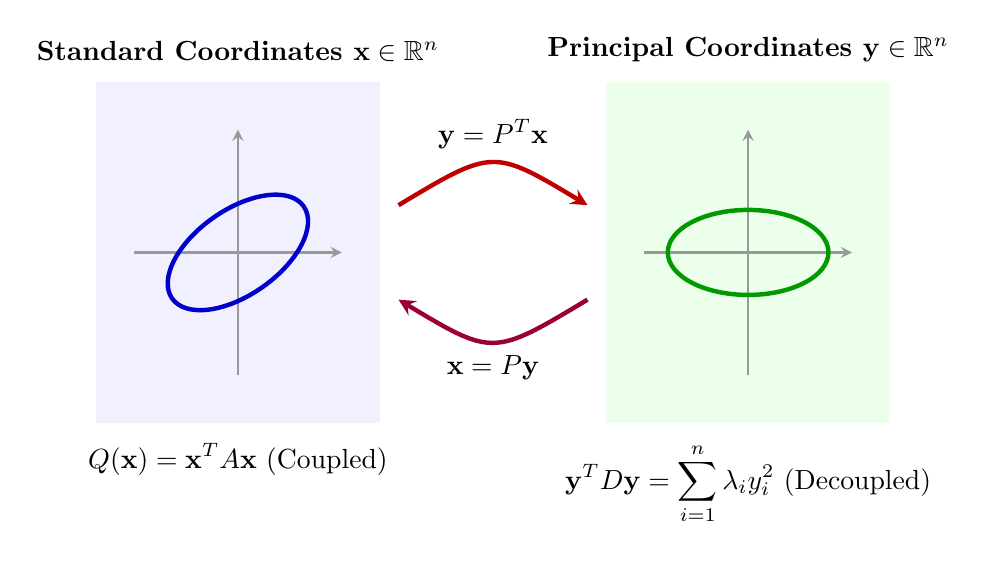
\begin{tikzpicture}[scale=1.2]
    % 1. Background fills
    \fill[blue!6] (-4.2, -1.8) rectangle (-1.2, 1.8);
    \fill[green!8] (1.2, -1.8) rectangle (4.2, 1.8);
    
    % 2. Coordinate Axes inside boxes
    \draw[->, >=stealth, gray!80, thick] (-3.8, 0) -- (-1.6, 0);
    \draw[->, >=stealth, gray!80, thick] (-2.7, -1.3) -- (-2.7, 1.3);
    
    \draw[->, >=stealth, gray!80, thick] (1.6, 0) -- (3.8, 0);
    \draw[->, >=stealth, gray!80, thick] (2.7, -1.3) -- (2.7, 1.3);
    
    % 3. Primary Plots and Mapping Arrows
    \draw[ultra thick, blue!80!black, rotate around={35:(-2.7,0)}] (-2.7,0) ellipse (0.85 and 0.45);
    \draw[ultra thick, green!60!black] (2.7,0) ellipse (0.85 and 0.45);
    
    \draw[->, >=stealth, ultra thick, red!75!black] (-1.0, 0.5) .. controls (0, 1.1) .. (1.0, 0.5);
    \draw[->, >=stealth, ultra thick, purple!80!black] (1.0, -0.5) .. controls (0, -1.1) .. (-1.0, -0.5);
    
    % 4. Labels and Nodes
    \node[above=4pt, black] at (-2.7, 1.8) {\textbf{Standard Coordinates $\mathbf{x} \in \mathbb{R}^n$}};
    \node[below=4pt, black] at (-2.7, -1.8) {$\displaystyle Q(\mathbf{x}) = \mathbf{x}^T A \mathbf{x}$ (Coupled)};
    
    \node[above=4pt, black] at (2.7, 1.8) {\textbf{Principal Coordinates $\mathbf{y} \in \mathbb{R}^n$}};
    \node[below=4pt, black] at (2.7, -1.8) {$\displaystyle \mathbf{y}^T D \mathbf{y} = \sum_{i=1}^n \lambda_i y_i^2$ (Decoupled)};
    
    \node[above=3pt, black] at (0, 0.9) {$\displaystyle \mathbf{y} = P^T \mathbf{x}$};
    \node[below=3pt, black] at (0, -0.9) {$\displaystyle \mathbf{x} = P \mathbf{y}$};
\end{tikzpicture}
\end{center}

\subsection{Backward and Forward Links in the Curriculum}
\begin{itemize}
    \item \textbf{Backward Links:} Section 7.2 is the direct payoff of Section 7.1 (Diagonalization of Symmetric Matrices). Without the guarantee that a symmetric matrix $A$ possesses $n$ real eigenvalues and an \textit{orthonormal} basis of eigenvectors ($P^T = P^{-1}$), a general invertible change of variable $\mathbf{x} = P\mathbf{y}$ would replace $A$ by $P^T A P$, which is a congruence transformation ($P^T A P$) rather than a similarity transformation ($P^{-1} A P$). Only when $P$ is orthogonal do congruence and similarity coincide ($P^T A P = P^{-1} A P = D$)!
    \item \textbf{Forward Links:}
    \begin{enumerate}
        \item \textbf{Constrained Optimization (Section 7.3):} The Principal Axes Theorem is the exact mechanism used to prove that the maximum and minimum values of $\mathbf{x}^T A \mathbf{x}$ on the unit sphere $\|\mathbf{x}\| = 1$ are the largest and smallest eigenvalues $\lambda_1$ and $\lambda_n$ of $A$.
        \item \textbf{The Singular Value Decomposition (Section 7.4):} As proven in Exercise 33, for any $m \times n$ matrix $B$, the matrix $B^T B$ is symmetric and positive semidefinite. The singular values $\sigma_i = \sqrt{\lambda_i}$ of $B$ are defined directly via the quadratic form $\|B\mathbf{x}\|^2 = \mathbf{x}^T (B^T B) \mathbf{x}$!
        \item \textbf{Multivariable Calculus (Second-Derivative Hessian Test):} Near a critical point $\nabla f(\mathbf{x}_0) = \mathbf{0}$, the second-order Taylor approximation is $\Delta f \approx \frac{1}{2} \mathbf{h}^T H_f(\mathbf{x}_0) \mathbf{h}$, where $H_f(\mathbf{x}_0)$ is the symmetric Hessian matrix. Thus $\mathbf{x}_0$ is a strict local minimum if $H_f(\mathbf{x}_0)$ is positive definite, a strict local maximum if negative definite, and a saddle point if indefinite.
    \end{enumerate}
\end{itemize}

\newpage
% =========================================================================
% PART 6: ABSTRACT REAL-WORLD MODELING (AI, ML, & QUANT FINANCE)
% =========================================================================
\section{Abstract Real-World Modeling (AI, ML, \& Quant Finance)}

\subsection{Concrete Scenarios in Quantitative Finance and Machine Learning}
\begin{enumerate}
    \item \textbf{Quantitative Finance (Markowitz Mean-Variance Portfolio Optimization \& Risk Decomposition):}
    Given $n$ risky financial assets with random return vector $\mathbf{R} \in \mathbb{R}^n$ and covariance matrix $\Sigma = \mathbb{E}[(\mathbf{R} - \boldsymbol{\mu})(\mathbf{R} - \boldsymbol{\mu})^T]$, the variance of a portfolio with weight vector $\mathbf{w} \in \mathbb{R}^n$ is the quadratic form $Q(\mathbf{w}) = \mathbf{w}^T \Sigma \mathbf{w}$. Because variance cannot be negative, $\Sigma$ is always symmetric positive semidefinite (and positive definite if no asset is a redundant linear combination of others). Orthogonal diagonalization $\Sigma = P D P^T$ transforms correlated asset weights $\mathbf{w}$ into uncorrelated \textbf{principal risk factors} $\mathbf{y} = P^T \mathbf{w}$ (eigen-portfolios), decomposing total portfolio variance into an additive sum of orthogonal factor variances $\sum_{i=1}^n \lambda_i y_i^2$.
    
    \item \textbf{Statistical Learning Theory \& Generative AI (Mahalanobis Distance and Multivariate Gaussian Flows):}
    The probability density function of an $n$-dimensional Gaussian distribution $\mathcal{N}(\boldsymbol{\mu}, \Sigma)$ is governed by the precision quadratic form:
    \[
    p(\mathbf{x}) = \frac{1}{(2\pi)^{n/2} (\det \Sigma)^{1/2}} \exp\left( -\frac{1}{2} (\mathbf{x} - \boldsymbol{\mu})^T \Sigma^{-1} (\mathbf{x} - \boldsymbol{\mu}) \right)
    \]
    By Exercise 36, since $\Sigma$ is positive definite, the precision matrix $\Sigma^{-1}$ is also symmetric positive definite. The level surfaces of constant probability density are concentric hyper-ellipsoids $(\mathbf{x} - \boldsymbol{\mu})^T \Sigma^{-1} (\mathbf{x} - \boldsymbol{\mu}) = c^2$. Furthermore, by Exercise 34 and the Cholesky factorization $\Sigma = R^T R$ (or spectral square root $\Sigma = B^2$), Generative AI models (such as Variational Autoencoders and Diffusion Models) apply the "reparameterization trick" $\mathbf{x} = \boldsymbol{\mu} + R^T \mathbf{z}$ to transform standard isotropic white noise $\mathbf{z} \sim \mathcal{N}(\mathbf{0}, I_n)$ into correlated data distributions.
    
    \item \textbf{Deep Learning Optimization (Hessian Curvature, Saddle Points, and Natural Gradient Descent):}
    When training a deep neural network with parameter vector $\boldsymbol{\theta} \in \mathbb{R}^d$ and loss function $\mathcal{L}(\boldsymbol{\theta})$, the local geometry around a stationary point $\nabla \mathcal{L}(\boldsymbol{\theta}^*) = \mathbf{0}$ is dictated by the quadratic form $\delta \boldsymbol{\theta}^T \nabla^2 \mathcal{L}(\boldsymbol{\theta}^*) \delta \boldsymbol{\theta}$. In high-dimensional non-convex loss landscapes, critical points are overwhelmingly \textbf{indefinite} saddle points (having both positive and negative eigenvalues) rather than local minima. Second-order optimizers (such as Kronecker-Factored Approximate Curvature, K-FAC) precondition the gradient using a positive definite quadratic form approximation (the Fisher Information Matrix) to scale step sizes inversely by the principal curvatures $\lambda_i$.
\end{enumerate}

\subsection{Rigorous Mathematical Model: Statistical Arbitrage \& Principal Factor Risk Budgeting}
Let $(\Omega, \mathcal{F}, \mathbb{P})$ be a probability space supporting an $n$-dimensional vector of excess asset returns $\mathbf{R} : \Omega \to \mathbb{R}^n$ with mean vector $\boldsymbol{\mu} = \mathbb{E}[\mathbf{R}] \in \mathbb{R}^n$ and covariance matrix $\Sigma = \operatorname{Cov}(\mathbf{R}) = \mathbb{E}[(\mathbf{R} - \boldsymbol{\mu})(\mathbf{R} - \boldsymbol{\mu})^T] \in \mathbb{R}^{n \times n}$.

\textbf{Proposition 1 (Positive Definiteness of Nonsingular Covariance):}
For any portfolio weight vector $\mathbf{w} \in \mathbb{R}^n$, the portfolio return is the random variable $R_p = \mathbf{w}^T \mathbf{R}$, and its variance is the quadratic form:
\[
\operatorname{Var}(R_p) = \mathbb{E}\left[ (\mathbf{w}^T (\mathbf{R} - \boldsymbol{\mu}))^2 \right] = \mathbb{E}\left[ \mathbf{w}^T (\mathbf{R} - \boldsymbol{\mu})(\mathbf{R} - \boldsymbol{\mu})^T \mathbf{w} \right] = \mathbf{w}^T \Sigma \mathbf{w} \ge 0
\]
Assuming no non-trivial risk-free linear combination of risky assets exists ($\mathbb{P}(\mathbf{w}^T(\mathbf{R}-\boldsymbol{\mu}) = 0) < 1$ for all $\mathbf{w} \neq \mathbf{0}$), $\Sigma$ is strictly positive definite ($\mathbf{w}^T \Sigma \mathbf{w} > 0$ for all $\mathbf{w} \neq \mathbf{0}$).

\textbf{Optimization Problem Formulation (Risk-Averse Mean-Variance Utility with $\ell_2$-Regularization):}
An institutional algorithmic trading desk seeks an optimal allocation $\mathbf{w}^* \in \mathbb{R}^n$ maximizing expected return penalized by quadratic portfolio variance and quadratic market-impact transaction cost $\gamma \|\mathbf{w}\|^2 = \gamma \mathbf{w}^T I_n \mathbf{w}$ ($\gamma > 0$, risk aversion $\kappa > 0$):
\[
\min_{\mathbf{w} \in \mathbb{R}^n} \mathcal{J}(\mathbf{w}) = \frac{1}{2} \mathbf{w}^T (\kappa \Sigma + \gamma I_n) \mathbf{w} - \boldsymbol{\mu}^T \mathbf{w}
\]
\textbf{Spectral Solution via Principal Axes:}
\begin{enumerate}
    \item By Exercise 35, since $\kappa \Sigma$ and $\gamma I_n$ are symmetric positive definite, the regularized risk matrix $A = \kappa \Sigma + \gamma I_n$ is strictly positive definite, guaranteeing that $\mathcal{J}(\mathbf{w})$ is strictly convex and possesses a unique global minimum.
    \item By the Principal Axes Theorem (Theorem 4), there exists an orthogonal matrix $P = \begin{bmatrix} \mathbf{u}_1 & \dots & \mathbf{u}_n \end{bmatrix}$ of orthonormal eigen-portfolios of $\Sigma$ such that $\Sigma = P D P^T$ with $D = \operatorname{diag}(\lambda_1, \dots, \lambda_n)$ ($\lambda_i > 0$).
    \item Applying the orthogonal change of variable $\mathbf{w} = P\mathbf{y}$ (where $\mathbf{y} = P^T \mathbf{w}$ represents allocations to the mutually uncorrelated principal eigen-portfolios) and defining $\tilde{\boldsymbol{\mu}} = P^T \boldsymbol{\mu}$ (expected returns of the eigen-portfolios), the objective function decouples completely into $n$ independent scalar quadratic optimizations:
    \[
    \mathcal{J}(P\mathbf{y}) = \frac{1}{2} \mathbf{y}^T P^T (\kappa \Sigma + \gamma I_n) P \mathbf{y} - (P^T \boldsymbol{\mu})^T \mathbf{y} = \sum_{i=1}^n \left( \frac{1}{2}(\kappa \lambda_i + \gamma) y_i^2 - \tilde{\mu}_i y_i \right)
    \]
    \item Differentiating with respect to each principal coordinate $y_i$ and setting to zero immediately yields the optimal allocation along each principal axis:
    \[
    y_i^* = \frac{\tilde{\mu}_i}{\kappa \lambda_i + \gamma} = \frac{\mathbf{u}_i^T \boldsymbol{\mu}}{\kappa \lambda_i + \gamma}, \quad \text{and hence} \quad \mathbf{w}^* = P\mathbf{y}^* = \sum_{i=1}^n \left( \frac{\mathbf{u}_i^T \boldsymbol{\mu}}{\kappa \lambda_i + \gamma} \right) \mathbf{u}_i
    \]
\end{enumerate}
This spectral formula provides profound quantitative intuition: the optimal weight allocated to the $i$-th principal axis $\mathbf{u}_i$ is directly proportional to its expected return $\mathbf{u}_i^T \boldsymbol{\mu}$ and inversely proportional to its regularized principal eigenvalue $\kappa \lambda_i + \gamma$.

\newpage
% =========================================================================
% PART 7: COMMON VARIATIONS AND UNTESTED CONCEPTS
% =========================================================================
\section{Common Variations and Untested Concepts}

While the assigned homework thoroughly tests matrix construction, orthogonal diagonalization, eigenvalue classification, and basic theoretical properties, standard linear algebra exams and advanced curricula frequently test three closely related variations that were not explicitly worked out in the exercises.

\subsection{Concept 1: Sylvester's Criterion (Leading Principal Minors Test)}
Finding all eigenvalues of an $n \times n$ matrix for $n \ge 3$ purely to check whether $A$ is positive definite or negative definite is computationally expensive. \textbf{Sylvester's Criterion} generalizes the $2 \times 2$ determinant test from Exercises 31--32 to any $n \times n$ symmetric matrix $A$ without computing a single eigenvalue!

\begin{theorem}[Sylvester's Criterion]
Let $A$ be an $n \times n$ symmetric matrix, and for each $k = 1, 2, \dots, n$, let $\Delta_k = \det(A_k)$ denote the $k$-th \textbf{leading principal minor} (the determinant of the top-left $k \times k$ submatrix $A_k$ of $A$).
\begin{enumerate}[label=\alph*.]
    \item $A$ is \textbf{positive definite} if and only if every leading principal minor is strictly positive:
    \[
    \Delta_1 > 0, \quad \Delta_2 > 0, \quad \Delta_3 > 0, \quad \dots, \quad \Delta_n > 0
    \]
    \item $A$ is \textbf{negative definite} if and only if the leading principal minors alternate in sign starting with $\Delta_1 < 0$:
    \[
    \Delta_1 < 0, \quad \Delta_2 > 0, \quad \Delta_3 < 0, \quad \dots, \quad (-1)^k \Delta_k > 0 \quad (\text{for } k = 1, \dots, n)
    \]
\end{enumerate}
\end{theorem}

\begin{example}[Applying Sylvester's Criterion to a $3 \times 3$ Quadratic Form]
Classify $Q(\mathbf{x}) = 3x_1^2 + 2x_2^2 + x_3^2 + 4x_1x_2 + 4x_2x_3$ (from Example 6) without finding eigenvalues.

\textbf{Solution:} The symmetric matrix is $A = \begin{bmatrix} 3 & 2 & 0 \\ 2 & 2 & 2 \\ 0 & 2 & 1 \end{bmatrix}$. We compute the leading principal minors:
\[
\Delta_1 = 3 > 0, \quad \Delta_2 = \det \begin{bmatrix} 3 & 2 \\ 2 & 2 \end{bmatrix} = 6 - 4 = 2 > 0, \quad \Delta_3 = \det(A) = 3(2 - 4) - 2(2 - 0) = -6 - 4 = -10 < 0
\]
Since $\Delta_3 = \det(A) = \lambda_1\lambda_2\lambda_3 = -10 < 0$ while $\Delta_1 > 0$, $A$ cannot have all positive or all negative eigenvalues; it must have both positive and negative eigenvalues, so $Q$ is \textbf{indefinite}.
\end{example}

\subsection{Concept 2: Explicit Computation of the Cholesky Factorization ($A = R^T R$)}
The Numerical Notes on page 454 and Exercise 29 introduce the Cholesky factorization $A = R^T R$, where $R$ is upper triangular with positive diagonal entries, as the fastest numerical test for positive definiteness. However, no exercise asked you to explicitly compute $R$.

\begin{example}[Computing a Cholesky Factorization]
Find the Cholesky factorization $A = R^T R$ for the positive definite matrix $A = \begin{bmatrix} 4 & -2 & 6 \\ -2 & 10 & -3 \\ 6 & -3 & 25 \end{bmatrix}$.

\textbf{Solution:} Let $R = \begin{bmatrix} r_{11} & r_{12} & r_{13} \\ 0 & r_{22} & r_{23} \\ 0 & 0 & r_{33} \end{bmatrix}$ with $r_{ii} > 0$. Equating $R^T R = A$:
\[
\begin{bmatrix} r_{11} & 0 & 0 \\ r_{12} & r_{22} & 0 \\ r_{13} & r_{23} & r_{33} \end{bmatrix} \begin{bmatrix} r_{11} & r_{12} & r_{13} \\ 0 & r_{22} & r_{23} \\ 0 & 0 & r_{33} \end{bmatrix} = \begin{bmatrix} r_{11}^2 & r_{11}r_{12} & r_{11}r_{13} \\ r_{11}r_{12} & r_{12}^2 + r_{22}^2 & r_{12}r_{13} + r_{22}r_{23} \\ r_{11}r_{13} & r_{12}r_{13} + r_{22}r_{23} & r_{13}^2 + r_{23}^2 + r_{33}^2 \end{bmatrix} = \begin{bmatrix} 4 & -2 & 6 \\ -2 & 10 & -3 \\ 6 & -3 & 25 \end{bmatrix}
\]
Solving row by row:
\begin{itemize}
    \item Row 1: $r_{11}^2 = 4 \implies r_{11} = 2$; \quad $2r_{12} = -2 \implies r_{12} = -1$; \quad $2r_{13} = 6 \implies r_{13} = 3$.
    \item Row 2: $(-1)^2 + r_{22}^2 = 10 \implies r_{22}^2 = 9 \implies r_{22} = 3$; \quad $(-1)(3) + 3r_{23} = -3 \implies r_{23} = 0$.
    \item Row 3: $3^2 + 0^2 + r_{33}^2 = 25 \implies r_{33}^2 = 16 \implies r_{33} = 4$.
\end{itemize}
Thus $R = \begin{bmatrix} 2 & -1 & 3 \\ 0 & 3 & 0 \\ 0 & 0 & 4 \end{bmatrix}$, and $\mathbf{x}^T A \mathbf{x} = \|R\mathbf{x}\|^2 = (2x_1 - x_2 + 3x_3)^2 + (3x_2)^2 + (4x_3)^2 > 0$ for all $\mathbf{x} \neq \mathbf{0}$.
\end{example}

\subsection{Concept 3: Geometric Identification and Sketching of Conic Sections $\mathbf{x}^T A \mathbf{x} = c$}
Pages 451--452 explain how the principal axes identify the exact geometry (semi-major and semi-minor axes, and rotation angle) of a conic section $\mathbf{x}^T A \mathbf{x} = c$.

\begin{example}[Identifying Semi-Axes of a Rotated Ellipse]
Identify the curve $6x_1^2 - 4x_1x_2 + 3x_2^2 = 14$ and find the lengths and directions of its semi-axes.

\textbf{Solution:} From Exercise 9, the orthogonal change of variable $\mathbf{x} = P\mathbf{y}$ with $P = \begin{bmatrix} 2/\sqrt{5} & 1/\sqrt{5} \\ -1/\sqrt{5} & 2/\sqrt{5} \end{bmatrix}$ transforms $6x_1^2 - 4x_1x_2 + 3x_2^2 = 14$ into:
\[
7y_1^2 + 2y_2^2 = 14 \quad \Longleftrightarrow \quad \frac{y_1^2}{2} + \frac{y_2^2}{7} = 1 \quad \Longleftrightarrow \quad \frac{y_1^2}{(\sqrt{2})^2} + \frac{y_2^2}{(\sqrt{7})^2} = 1
\]
Thus the curve is an \textbf{ellipse} with semi-minor axis of length $a = \sqrt{2}$ along the principal axis $\mathbf{u}_1 = \begin{bmatrix} 2/\sqrt{5} \\ -1/\sqrt{5} \end{bmatrix}$ and semi-major axis of length $b = \sqrt{7}$ along the principal axis $\mathbf{u}_2 = \begin{bmatrix} 1/\sqrt{5} \\ 2/\sqrt{5} \end{bmatrix}$.
\end{example}

\newpage
% =========================================================================
% PART 8: ADVANCED DIAGNOSTIC TESTING: "FIND THE FLAW"
% =========================================================================
\section{Advanced Diagnostic Testing: ``Find the Flaw''}

For each of the five problems below, a seemingly complete solution is presented that contains a \textbf{single, subtle, yet fatal mathematical flaw}. First try to spot the error yourself, then review the diagnostic grading analysis underneath.

\medskip\hrule\medskip

\subsection*{Diagnostic Problem 1: Matrix Construction and Classification}
\textbf{Problem:} Find the symmetric matrix $A$ of the quadratic form $Q(\mathbf{x}) = 2x_1^2 - 4x_1x_2 + 5x_2^2$ on $\mathbb{R}^2$ and determine its eigenvalues.

\textbf{Flawed Solution:}
\begin{enumerate}
    \item Reading the coefficients from $Q(\mathbf{x}) = 2x_1^2 - 4x_1x_2 + 5x_2^2$, we place $2$ and $5$ on the main diagonal and $-4$ in the off-diagonal positions to make $A$ symmetric:
    \[
    A = \begin{bmatrix} 2 & -4 \\ -4 & 5 \end{bmatrix}
    \]
    \item Solving the characteristic equation $\det(A - \lambda I) = 0$:
    \[
    (2 - \lambda)(5 - \lambda) - (-4)^2 = \lambda^2 - 7\lambda + 10 - 16 = \lambda^2 - 7\lambda - 6 = 0
    \]
    \item By the quadratic formula, the eigenvalues are $\lambda = \frac{7 \pm \sqrt{73}}{2}$. Since one eigenvalue is positive and the other is negative, $Q(\mathbf{x})$ is indefinite.
\end{enumerate}

\textbf{Grader's Diagnostic Analysis:}
\begin{itemize}
    \item \textbf{The Flaw:} In Step 1, the cross-product coefficient $-4$ was placed directly into $a_{12}$ and $a_{21}$ without dividing by $2$ (which corresponds to $2x_1^2 - 8x_1x_2 + 5x_2^2$ instead of $2x_1^2 - 4x_1x_2 + 5x_2^2$).
    \item \textbf{Correct Step and Final Solution:} Splitting the $-4x_1x_2$ term evenly gives $a_{12} = a_{21} = -4/2 = -2$, so
    \[
    A = \begin{bmatrix} 2 & -2 \\ -2 & 5 \end{bmatrix}
    \]
    The characteristic equation is $(2-\lambda)(5-\lambda) - (-2)^2 = \lambda^2 - 7\lambda + 6 = (\lambda - 6)(\lambda - 1) = 0$. The true eigenvalues are $\lambda_1 = 6$ and $\lambda_2 = 1$, and $Q(\mathbf{x})$ is \textbf{positive definite}.
\end{itemize}

\medskip\hrule\medskip

\subsection*{Diagnostic Problem 2: Principal Axes Change of Variable}
\textbf{Problem:} Find the orthogonal matrix $P$ and the new quadratic form $\mathbf{y}^T D \mathbf{y}$ that eliminates the cross-product term from $Q(\mathbf{x}) = 5x_1^2 - 4x_1x_2 + 8x_2^2$ using $\mathbf{x} = P\mathbf{y}$, and evaluate $Q(\mathbf{x})$ at $\mathbf{y} = \begin{bmatrix} 1 \\ 0 \end{bmatrix}$.

\textbf{Flawed Solution:}
\begin{enumerate}
    \item The symmetric matrix of the quadratic form is $A = \begin{bmatrix} 5 & -2 \\ -2 & 8 \end{bmatrix}$.
    \item The characteristic equation is $(5-\lambda)(8-\lambda) - 4 = \lambda^2 - 13\lambda + 36 = (\lambda - 9)(\lambda - 4) = 0$, giving eigenvalues $\lambda_1 = 9$ and $\lambda_2 = 4$.
    \item For $\lambda_1 = 9$, $(A - 9I)\mathbf{v} = \begin{bmatrix} -4 & -2 \\ -2 & -1 \end{bmatrix}\mathbf{v} = \mathbf{0} \implies \mathbf{v}_1 = \begin{bmatrix} 1 \\ -2 \end{bmatrix}$.
    For $\lambda_2 = 4$, $(A - 4I)\mathbf{v} = \begin{bmatrix} 1 & -2 \\ -2 & 4 \end{bmatrix}\mathbf{v} = \mathbf{0} \implies \mathbf{v}_2 = \begin{bmatrix} 2 \\ 1 \end{bmatrix}$.
    \item Since $\mathbf{v}_1 \cdot \mathbf{v}_2 = (1)(2) + (-2)(1) = 0$, the eigenvectors are orthogonal. Setting $P = \begin{bmatrix} 1 & 2 \\ -2 & 1 \end{bmatrix}$, the change of variable $\mathbf{x} = P\mathbf{y}$ gives $\mathbf{y}^T D \mathbf{y} = 9y_1^2 + 4y_2^2$, so at $\mathbf{y} = \begin{bmatrix} 1 \\ 0 \end{bmatrix}$ (i.e., $\mathbf{x} = P\mathbf{y} = \begin{bmatrix} 1 \\ -2 \end{bmatrix}$), $Q(\mathbf{x}) = 9(1)^2 + 4(0)^2 = 9$.
\end{enumerate}

\textbf{Grader's Diagnostic Analysis:}
\begin{itemize}
    \item \textbf{The Flaw:} In Step 4, the orthogonal eigenvectors $\mathbf{v}_1$ and $\mathbf{v}_2$ were not normalized to unit length before forming $P$, so $P$ is not an orthogonal matrix ($P^T P = 5I_2 \neq I_2$, and $P^T A P = \begin{bmatrix} 45 & 0 \\ 0 & 20 \end{bmatrix} \neq \begin{bmatrix} 9 & 0 \\ 0 & 4 \end{bmatrix}$).
    \item \textbf{Correct Step and Final Solution:} Dividing each eigenvector by $\|\mathbf{v}_i\| = \sqrt{5}$ gives the orthogonal matrix
    \[
    P = \begin{bmatrix} 1/\sqrt{5} & 2/\sqrt{5} \\ -2/\sqrt{5} & 1/\sqrt{5} \end{bmatrix}
    \]
    With this normalized $P$, $\mathbf{x} = P\mathbf{y}$ truly gives $Q(\mathbf{x}) = 9y_1^2 + 4y_2^2$, and at $\mathbf{y} = \begin{bmatrix} 1 \\ 0 \end{bmatrix}$ (which corresponds to the unit vector $\mathbf{x} = \begin{bmatrix} 1/\sqrt{5} \\ -2/\sqrt{5} \end{bmatrix}$), $Q(\mathbf{x}) = 5(1/5) - 4(-2/5) + 8(4/5) = 45/5 = 9$. (Whereas for the unnormalized $\mathbf{x} = \begin{bmatrix} 1 \\ -2 \end{bmatrix}$, $Q(1, -2) = 5(1) - 4(-2) + 8(4) = 45$.)
\end{itemize}

\medskip\hrule\medskip

\subsection*{Diagnostic Problem 3: Definiteness Classification from Determinant Alone}
\textbf{Problem:} Classify the quadratic form $Q(\mathbf{x}) = -3x_1^2 + 4x_1x_2 - 2x_2^2$ on $\mathbb{R}^2$.

\textbf{Flawed Solution:}
\begin{enumerate}
    \item The symmetric matrix of the quadratic form is $A = \begin{bmatrix} -3 & 2 \\ 2 & -2 \end{bmatrix}$.
    \item We compute the determinant of $A$:
    \[
    \det A = (-3)(-2) - (2)^2 = 6 - 4 = 2 > 0
    \]
    \item Since $\det A = \lambda_1 \lambda_2 = 2 > 0$, the product of the eigenvalues is strictly positive, so $Q(\mathbf{x})$ is positive definite.
\end{enumerate}

\textbf{Grader's Diagnostic Analysis:}
\begin{itemize}
    \item \textbf{The Flaw:} In Step 3, $\det A = \lambda_1 \lambda_2 > 0$ only implies that $\lambda_1$ and $\lambda_2$ have the \textit{same sign} (either both positive or both negative), not that they are positive; one must also check the sign of $a_{11}$ (or the trace $\lambda_1 + \lambda_2 = a + d$).
    \item \textbf{Correct Step and Final Solution:} Since $\det A = 2 > 0$ and $a = -3 < 0$ (with $\operatorname{tr}(A) = \lambda_1 + \lambda_2 = -5 < 0$), both eigenvalues are strictly negative, so by Exercise 32(b) $Q(\mathbf{x})$ is \textbf{negative definite}.
\end{itemize}

\medskip\hrule\medskip

\subsection*{Diagnostic Problem 4: Ordering Mismatch Between $P$ and $D$}
\textbf{Problem:} For $Q(\mathbf{x}) = 2x_1^2 + 4x_1x_2 + 5x_2^2$, construct $P$ and state the new quadratic form $\mathbf{y}^T D \mathbf{y}$ under $\mathbf{x} = P\mathbf{y}$.

\textbf{Flawed Solution:}
\begin{enumerate}
    \item The matrix is $A = \begin{bmatrix} 2 & 2 \\ 2 & 5 \end{bmatrix}$, with characteristic polynomial $(2-\lambda)(5-\lambda) - 4 = \lambda^2 - 7\lambda + 6 = (\lambda - 6)(\lambda - 1) = 0$. The eigenvalues in decreasing order are $\lambda_1 = 6$ and $\lambda_2 = 1$.
    \item Finding unit eigenvectors:
    \begin{itemize}
        \item For $\lambda = 1$: $(A - I)\mathbf{v} = \begin{bmatrix} 1 & 2 \\ 2 & 4 \end{bmatrix}\mathbf{v} = \mathbf{0} \implies \mathbf{u}_1 = \begin{bmatrix} 2/\sqrt{5} \\ -1/\sqrt{5} \end{bmatrix}$.
        \item For $\lambda = 6$: $(A - 6I)\mathbf{v} = \begin{bmatrix} -4 & 2 \\ 2 & -1 \end{bmatrix}\mathbf{v} = \mathbf{0} \implies \mathbf{u}_2 = \begin{bmatrix} 1/\sqrt{5} \\ 2/\sqrt{5} \end{bmatrix}$.
    \end{itemize}
    \item Placing $\mathbf{u}_1$ and $\mathbf{u}_2$ as the columns of $P$ and using $\lambda_1 = 6, \lambda_2 = 1$, we get:
    \[
    P = \begin{bmatrix} 2/\sqrt{5} & 1/\sqrt{5} \\ -1/\sqrt{5} & 2/\sqrt{5} \end{bmatrix} \quad \text{and} \quad Q(P\mathbf{y}) = 6y_1^2 + y_2^2
    \]
\end{enumerate}

\textbf{Grader's Diagnostic Analysis:}
\begin{itemize}
    \item \textbf{The Flaw:} In Step 3, the first column of $P$ was chosen to be the eigenvector for $\lambda = 1$ while the first coefficient in the new quadratic form was written as $6$ (the eigenvalue for the second column of $P$).
    \item \textbf{Correct Step and Final Solution:} The order of the eigenvalues in $\mathbf{y}^T D \mathbf{y}$ must match the order of the eigenvector columns in $P$:
    \[
    \text{Either } P = \begin{bmatrix} 1/\sqrt{5} & 2/\sqrt{5} \\ 2/\sqrt{5} & -1/\sqrt{5} \end{bmatrix} \text{ with } 6y_1^2 + y_2^2, \quad \text{or } P = \begin{bmatrix} 2/\sqrt{5} & 1/\sqrt{5} \\ -1/\sqrt{5} & 2/\sqrt{5} \end{bmatrix} \text{ with } y_1^2 + 6y_2^2.
    \]
\end{itemize}

\medskip\hrule\medskip

\subsection*{Diagnostic Problem 5: Non-Orthogonal Eigenvectors in a Repeated Eigenspace}
\textbf{Problem:} Let $A = \begin{bmatrix} 5 & 2 & 2 \\ 2 & 5 & 2 \\ 2 & 2 & 5 \end{bmatrix}$. Given that the eigenvalues of $A$ are $\lambda_1 = 9$ and $\lambda_2 = \lambda_3 = 3$, find an orthogonal matrix $P$ such that $\mathbf{x} = P\mathbf{y}$ transforms $\mathbf{x}^T A \mathbf{x}$ into $9y_1^2 + 3y_2^2 + 3y_3^2$.

\textbf{Flawed Solution:}
\begin{enumerate}
    \item For $\lambda_1 = 9$, $(A - 9I)\mathbf{v} = \begin{bmatrix} -4 & 2 & 2 \\ 2 & -4 & 2 \\ 2 & 2 & -4 \end{bmatrix}\mathbf{v} = \mathbf{0} \implies x_1 = x_2 = x_3$, so $\mathbf{u}_1 = \begin{bmatrix} 1/\sqrt{3} \\ 1/\sqrt{3} \\ 1/\sqrt{3} \end{bmatrix}$.
    \item For $\lambda_2 = \lambda_3 = 3$, $(A - 3I)\mathbf{v} = \begin{bmatrix} 2 & 2 & 2 \\ 2 & 2 & 2 \\ 2 & 2 & 2 \end{bmatrix}\mathbf{v} = \mathbf{0} \implies x_1 + x_2 + x_3 = 0$.
    Two linearly independent basis vectors for this $2$-dimensional eigenspace are $\mathbf{v}_2 = \begin{bmatrix} 1 \\ -1 \\ 0 \end{bmatrix}$ and $\mathbf{v}_3 = \begin{bmatrix} 1 \\ 0 \\ -1 \end{bmatrix}$.
    \item Normalizing $\mathbf{v}_2$ and $\mathbf{v}_3$ gives $\mathbf{u}_2 = \begin{bmatrix} 1/\sqrt{2} \\ -1/\sqrt{2} \\ 0 \end{bmatrix}$ and $\mathbf{u}_3 = \begin{bmatrix} 1/\sqrt{2} \\ 0 \\ -1/\sqrt{2} \end{bmatrix}$. Thus the orthogonal matrix is:
    \[
    P = \begin{bmatrix} 1/\sqrt{3} & 1/\sqrt{2} & 1/\sqrt{2} \\ 1/\sqrt{3} & -1/\sqrt{2} & 0 \\ 1/\sqrt{3} & 0 & -1/\sqrt{2} \end{bmatrix}
    \]
\end{enumerate}

\textbf{Grader's Diagnostic Analysis:}
\begin{itemize}
    \item \textbf{The Flaw:} In Step 2 and Step 3, because $\lambda = 3$ is a repeated eigenvalue of multiplicity $2$, two linearly independent eigenvectors $\mathbf{v}_2$ and $\mathbf{v}_3$ from the \textit{same} eigenspace are not automatically orthogonal ($\mathbf{v}_2 \cdot \mathbf{v}_3 = 1 \neq 0$), so the resulting matrix $P$ is not orthogonal!
    \item \textbf{Correct Step and Final Solution:} We must apply the Gram-Schmidt process to $\{\mathbf{v}_2, \mathbf{v}_3\}$ (or choose $\mathbf{v}_3$ orthogonal to both $\mathbf{u}_1$ and $\mathbf{v}_2$):
    \[
    \mathbf{w}_3 = \mathbf{v}_3 - \frac{\mathbf{v}_3 \cdot \mathbf{v}_2}{\mathbf{v}_2 \cdot \mathbf{v}_2}\mathbf{v}_2 = \begin{bmatrix} 1 \\ 0 \\ -1 \end{bmatrix} - \frac{1}{2}\begin{bmatrix} 1 \\ -1 \\ 0 \end{bmatrix} = \begin{bmatrix} 1/2 \\ 1/2 \\ -1 \end{bmatrix} \propto \begin{bmatrix} 1 \\ 1 \\ -2 \end{bmatrix}
    \]
    Normalizing $\mathbf{w}_3$ yields $\mathbf{u}_3 = \begin{bmatrix} 1/\sqrt{6} \\ 1/\sqrt{6} \\ -2/\sqrt{6} \end{bmatrix}$, and the true orthogonal matrix is:
    \[
    P = \begin{bmatrix} 1/\sqrt{3} & 1/\sqrt{2} & 1/\sqrt{6} \\ 1/\sqrt{3} & -1/\sqrt{2} & 1/\sqrt{6} \\ 1/\sqrt{3} & 0 & -2/\sqrt{6} \end{bmatrix}
    \]
\end{itemize}

\end{document}